% Když budete cokoli psát: ukládejte starší verze vždy odděleně, abyste se 
% k nim mohli kdykoli vrátit. Kusy textu, které jste se rozhodli nepoužít, taky ukládejte do zvláštního souboru. Smazat se to dá vždycky, ale psát to znova je opruz. 

% A POŘÁD ZÁLOHUJTE. POŘÁD !!!

% priklady update
% proxy lip
% libenjoy -> reference
% libenjoy neni prilis rozsahla

\documentclass[12pt, a4paper, oneside]{article} 
% velikost písma, stránky, typ dokumentu -- detaily viz literatura

\usepackage{czech} % nastavení češtiny
%\usepackage[latin2]{inputenc}
%\usepackage[cp1250]{inputenc} % pro win1250
\usepackage[center]{caption} 
\usepackage[utf8]{inputenc}
\usepackage{wrapfig} % nastavení obtékání textu
\usepackage{graphicx,amsmath} % nastavení grafiky, matematiky
\usepackage{subfig} % více obrázků vedle sebe 
\usepackage{float}
\usepackage{amsmath}
\usepackage{amssymb}
\usepackage{bbding}
\usepackage{enumitem}
\usepackage{breakurl}
\usepackage{pdflscape}
%\usepackage{indentfirst}

\usepackage{tocloft} %přidá tečky do obsahu ke kapitolám /sekcím 
\renewcommand{\cftsecdotsep}{\cftdotsep}

\usepackage[bookmarksopen,colorlinks,plainpages=false,linkcolor=black,urlcolor=blue,citecolor=black,filecolor=black,menucolor=black,unicode=true]{hyperref}

\urlstyle{rm}
%bookmarksopen -- open up bookmark tree 
%colorlinks -- zbarví odkazy (implicitně orámovaný nezbarvený text)
%urlcolor -- barva odkazů (implicitně magenta) 
%linkcolor=black -- barva odkazů v obsahu (implicitně red)


\usepackage{listings}
\usepackage{color}
\usepackage{minted}
\definecolor{lightgray}{RGB}{240,240,240}
\definecolor{darkgray}{rgb}{.4,.4,.4}
\definecolor{purple}{rgb}{0.65, 0.12, 0.82}
\definecolor{darkgreen}{RGB}{0,150,0}

\usemintedstyle{perldoc}
\newminted{js}{linenos=true, bgcolor=lightgray}

\lstdefinelanguage{JavaScript}{
  keywords={typeof, new, true, false, catch, function, return, null, catch, switch, var, if, in, while, do, else, case, break, for},
  keywordstyle=\color{blue}\bfseries,
  ndkeywords={class, export, boolean, throw, implements, import, this},
  ndkeywordstyle=\color{blue}\bfseries,
  identifierstyle=\color{black},
  sensitive=zr,
  comment=[l]{//},
  morecomment=[s]{/*}{*/},
  commentstyle=\color{darkgreen}\ttfamily,
  stringstyle=\color{red}\ttfamily,
  morestring=[b]',
  morestring=[b]"
}

\lstset{
   backgroundcolor=\color{lightgray},
   extendedchars=true,
   basicstyle=\footnotesize\ttfamily,
   showstringspaces=false,
   showspaces=false,
   numbers=left,
   numberstyle=\footnotesize,
   numbersep=9pt,
   tabsize=2,
   breaklines=true,
   showtabs=false,
   aboveskip=5mm,
   belowskip=7mm,
   captionpos=b
}

\renewcommand{\listingscaption}{Příklad}
\renewcommand{\listoflistingscaption}{Příklady}

% \usepackage{parskip} -- zapne americké odstavce v celé práci

\addtolength{\textwidth}{-2mm} 
\addtolength{\hoffset}{4mm}  % posun textu kvůli kroužkové vazbě  

\setlength{\intextsep}{5mm} % nastavení mezery okolo obrázků

% nastavení příkazu >\figcaption pro popis čehokoli, jako by to byly obrázky 
\makeatletter   
\newcommand\figcaption{\def\@captype{figure}\caption}
\makeatother

\renewcommand\refname{Literatura} 
%\def\bibname{PŘÍLOHA D: Reference}
%\renewcommand\bibname{PŘÍLOHA D: Reference}
% přejmenuje anglický název Reference na české Literatura


%\makeindex % příprava pro výrobu indexu (jestli ho chcete)

%%    VLNKA <fileinput>  KkSsVvZzOoUuAaIi        
% Defaultni  koncovka pro <fileinput> je  ".tex"
%FIXME: haze error
%\cstieon % Vypne chovani vlnky jako tvrde mezery v matematickem rezimu

%%%%%%%%%%%%%%%%%%%%%%%%%%%%%%%%%%%%%%%%%%%%%%%%%%%%%%%%%%%%%%%
%V PROSTŘEDÍ ROVNIC SE NESMÍ VYSKYTOVAT PRÁZDNÝ ŘÁDEK
%
%PROGRAMY VLNKA A CSINDEX SE MUSÍ SPUSTIT SAMOSTATNĚ
%%%%%%%%%%%%%%%%%%%%%%%%%%%%%%%%%%%%%%%%%%%%%%%%%%%%%%%%%%%%%%%

% definice příkazů 
\newcommand{\D}{\medskip \noindent} % nový odstavec v "americkém" formátování 
\newcommand{\B}{\textbf} %tučné písmo
\newcommand{\A}{\mathbf} %tučné písmo v matematickém režimu
\newcommand{\TO}{\ensuremath{\boldsymbol\Omega}} % tučný znak velké omega -- pro ohmy
\newcommand{\I}{\index}  % vytváří položku indexu (asi nepoužijete)
\newcommand{\Deg}[1][]{\ensuremath{{#1}^\circ}} % vysází značku stupně Celsia
\newcommand{\Def}{\footnotesize Definice: \normalsize}
\newcommand{\Pos}{\footnotesize Experiment: \normalsize}
\newcommand{\Odv}{\footnotesize Odvození: \normalsize}
\newcommand{\Vym}{\footnotesize Vymezení pojmu: \normalsize}
\newcommand{\Ob}{obrázek }
\newcommand{\It}{\textit}  % kurzíva
\newcommand{\M}{\mathrm}   % v prostředí rovnic nastaví normální písmo (místo kurzívy ) 
\newcommand{\F}{\footnotesize} % zmenšená velikost písma
\newcommand{\N}{\normalsize} % normální velikost písma
%\newcommand{\U}{\underline}  % podtržené písmo
\newcommand{\e}{\ensuremath} 
\newcommand{\Has}{\textcolor{green}{\CheckmarkBold}}
\newcommand{\NoHas}{\textcolor{red}{\XSolidBrush}}
% další příkaz se aplikuje, pouze, když jste v matematickém režimu

%\hyphenation{Pusť-me pla-tí hod-no-ty do-sa-dí-me za-da-né dal-ším}
% dělení slov, kdyby implicitní nevyhovovalo

\linespread{1.3} 
% řádkování 1,5x  
% použijete podle situace  

\unitlength=1mm % nastavení volby jednotek 

% konec hlavičky
%%%%%%%%%%%%%%%%%%%%%%%%%%%%%%%%%%%%%%%%%%%%%%%%%%%%%%%%%%%%%%%%%%%
%%%%%%%%%%%%%%%%%%%%%%%%%%%%%%%%%%%%%%%%%%%%%%%%%%%%%%%%%%%%%%%%%%%

\begin{document} % začátek textové části 

% titulní strana
\pagestyle{empty} % vynechá číslování
 
\voffset = -20mm % posun začátku textu výš
\enlargethispage{60mm} % zvětší oblast tisku pro tuto stránku   

\begin{center}
 
\Large \B{STŘEDOŠKOLSKÁ ODBORNÁ ČINNOST}

\vspace{60mm}

\huge %\LARGE
\B{LORRIS TOOLBOX \\ Sada nástrojů pro vývoj a~řízení robotů}
% na titulní straně může být stručnější, pokud je to potřeba  

\Large

\vspace{90mm}


\B{Vojtěch Boček} \\

\vspace{40mm}

\B{Brno 2013}


\end{center}

\newpage % konec titulní strany 
%%%%%%%%%%%%%%%%%%%%%%%%%%%%%%%%%%%%%%%%%%%%%%%%%%%%%%%%%%%%%%%%%%%%%%%%%%%

% vnitřní titulní strana
\voffset = -20mm % posun začátku textu výš
\enlargethispage{60mm} % zvětší oblast tisku pro tuto stránku   

\begin{center}

\Large \B{STŘEDOŠKOLSKÁ ODBORNÁ ČINNOST}  \\
\vspace{10mm}
 \normalsize 
\B{Obor SOČ: 18. Informatika}% číslo a název -- vyplníme spolu 

\vspace{45mm}

\LARGE %\huge 
\B{LORRIS TOOLBOX \\ Sada nástrojů pro vývoj a~řízení robotů}%SADA NÁSTORUJŮ PRO VÝVOJ A ŘÍZENÍ ROBOTŮ} 
\end{center}  
\large

\vspace{50mm}


\begin{tabbing}
\hspace{10mm} \= \hspace{30mm}  \=   \kill % nastavení zarážek 
  \> \B{Autor:}  \> \B{Vojtěch Boček}        \\[8mm] 
  \> \B{Škola:}   \> \B{SPŠ a~VOŠ technická, }     \\
  \>              \> \B{Sokolská 1, 602 00 Brno}    \\[8mm]

  \> \B{Konzultant:} \> \B {Jakub Streit} 
\end{tabbing}

\vspace{20mm}

\begin{center}
\B{Brno 2013}

\end{center}
\normalsize
%%%%%%%%%%%%%%%%%%%%%%%%%%%%%%%%%%%%%%%%%%%%%%%%%%%%%%%%%%%%%%%%%%%%%%%%%%%
\newpage  % Prohlášení o autorství  
\voffset = 0mm % posun začátku textu zpět

~ % musí to tu být, aby fungovala svislá mezera

\vspace{10mm}

\section*{Prohlášení}

Prohlašuji, že jsem svou práci vypracoval samostatně, použil jsem pouze podklady (literaturu, SW atd.) citované v~práci a~uvedené v~přiloženém seznamu a~postup při zpracování práce je v~souladu se zákonem č. 121/2000 Sb., o~právu autorském, o~právech souvisejících s~právem autorským a~o~změně některých zákonů (autorský zákon) v~platném znění. 
 
\vspace{20mm} 
 
\noindent V~Brně  dne: 6.3.2013 \hspace{50mm}                 podpis:   
 

%%%%%%%%%%%%%%%%%%%%%%%%%%%%%%%%%%%%%%%%%%%%%%%%%%%%%%%%%%%%%%%%%%%%%%%%%%%
\newpage   % Poděkování -- nepovinné 

~ % musí to tu být, aby fungovala svislá mezera
\vspace{100mm}

\section*{Poděkování}
Děkuji Jakubu Streitovi za rady, obětavou pomoc, velkou trpělivost a~podnětné připomínky poskytované během práce na tomto projektu, Martinu Vejnárovi za informace o programátoru Shupito, panu profesorovi Mgr. Miroslavu Burdovi za velkou pomoc s prací a v neposlední řadě Bc. Martinu Foučkovi za rady a pomoc při práci s Qt Frameworkem. Dále děkuji organizaci DDM Junior za poskytnutí podpory.

\D Tato práce byla vypracována za finanční podpory JMK a JCMM.

\begin{figure}[H]
\begin{center}

\includegraphics[width=\textwidth]{img/jcmm.png}
\end{center}
\end{figure}
 

%%%%%%%%%%%%%%%%%%%%%%%%%%%%%%%%%%%%%%%%%%%%%%%%%%%%%%%%%%%%%%%%%%%%%%%%%%%
\newpage   % Anotace 
~ % musí to tu být, aby fungovala svislá mezera
\vspace{-20mm}

\section*{Anotace}

Tato práce popisuje komplexní sadu nástrojů pro vývoj a ovládání libovolného zařízení schopného komunikovat po sériové lince nebo TCP socketu.

Protože se nejedná o jednoduchou aplikaci ani o jednostranně zaměřenou sadu nástrojů, protože se navíc celá sada průběžně rozrůstá a protože je rozsah a záběr použití všech funkcí a modulů této sady příliš velký, nelze ji stručně popsat v omezeném prostoru anotace.

Pro získání ucelenější představy o tom co vše lze pomocí sady Lorris dosáhnout, prosím nahlédněte do \hyperref[uvod]{úvodu práce}.

%Aplikace zastřešuje několik modulů. Každý modul je určen pro specifickou činnost -- parsování a zobrazování dat, programování mikročipů atd.

Hlavním přínosem tohoto softwarového balíku je, že urychluje, zpřehledňuje a hlavně výrazně zjednodušuje vývoj a testování aplikací pro mikročipy, typicky programování a řízení různých druhů robotů.

\D \B{Klíčová slova:} analýza binárních dat, programování a řízení robotů, vývoj pro mikrokontroléry, programování mikročipů

\section*{Annotation}

This work describes a complex set of tools designed for developement and control of any device capable of connecting to serial port or TCP socket.

Because Lorris isn't a simple application nor is it a toolbox focused on one narrow area of use, because the whole set is continuously growing and because scope of use for all features and modules of Lorris is too big, it is impossible to briefly describe it all in limited scope of annotation.

To get better notion of what can one achieve with Lorris, please refer to introductory chapter of this work (English version of this text is available on enclosed CD as PDF file).

Main asset of this software package is the ability to significantly speed-up and simplify developement and testing of various applications for microcontrollers, typically programming and controlling various kinds of robots.

\D \B{Key words:} binary data analysis, programming and control of robots, developement for microcontrollers, programming of microchips

\addtolength{\textheight}{30mm} % prodlouží následující stránku

%%%%%%%%%%%%%%%%%%%%%%%%%%%%%%%%%%%%%%%%%%%%%%%%%%%%%%%%%%%%%%%%%%%%%%%%%%%
\newpage
\pagestyle{plain}

\setlength{\voffset}{-20mm} % posune text/obrázek na této stránce nahoru
\setcounter{page}{1}  % nastaví čítač stránek znovu od jedné

\tableofcontents  % vysází obsah

\addtolength{\textheight}{-30mm} % zkrátí následující stránku
%%%%%%%%%%%%%%%%%%%%%%%%%%%%%%%%%%%%%%%%%%%%%%%%%%%%%%%%%%%%%%%%%%%%%%%%%%%
\newpage
\setlength{\voffset}{0mm} % posune text/obrázek na této stránce, kam patří
%\pagestyle{headings} % znovu zapne číslování
\pagestyle{plain}

\section*{Úvod}
\addcontentsline{toc}{section}{Úvod} % přidá položku úvod do obsahu
\label{uvod}
Lorris je rozsáhlá sada nástrojů, které mají společný cíl -- pomáhat při vývoji, ladění a řízení zejména robotů, ale i jiných elektronických zařízení. V této kapitole najdete stručně popsány nejdůležitější vlastnosti jednotlivých modulů a dále v práci jsou pak všechny moduly důkladně popsány v jednotlivých kapitolách.

\subsection*{Modul: analyzér}
\addcontentsline{toc}{subsection}{Modul: analyzér}
\begin{itemize} 
    \item Soustřeďuje se na zobrazování dat ze zařízení v grafické podobě.
    \item Analyzér pro zobrazování používá tzv. widgety -- malá \uv{okna}, která zobrazují určitou část dat.
    \item Widgety mají individuální nastavení a uživatel si je může umístit na libovolné místo na pracovní ploše.
    \item Lorris obsahuje několik typů widgetů, například \It{Číslo, Barva, Sloupcový bar, Kolo} (zobrazení úhlu v kružnici) či \It{Graf}.
    \item Pomocí widgetů lze sestavit rozhraní vyhovující prakticky jakémukoliv zařízení.
    \item Analyzér je ideální i pro snadné zobrazování dat z prvků, u kterých není vhodné jako výstup použít čísla -- například barevný senzor.
    \item Některé widgety mohou posílat data i směrem do zařízení. Díky tomu je možné kromě zobrazování dat jejich prostřednictvím zařízení i ovládat.
    \item Pozornost si zaslouží widget \uv{script}. Uživatel v něm může napsat vlastní script, který zpracovává příchozí data. Script může využít ostatní widgety a další části Lorris, díky tomu lze zobrazit i jinými způsoby interpretovat takřka jakákoliv data.
    \item Pomocí scriptu lze upravovat i samotnou sadu Lorris.
\end{itemize}

\subsection*{Modul: programátor}
\addcontentsline{toc}{subsection}{Modul: programátor}
\begin{itemize}
    \item Grafické rozhraní pro několik typů bootloaderů a programátorů pro mikročipy.
    \item Dokáže do čipu zapistovat program, číst a mazat paměť čipu nebo programovat pojistky.
    \item Oficiální GUI k programátoru Shupito.
    \item Shupito je programátor mikrokontrolérů. Na jeden konec programátoru se připojí čip, na druhý počítač -- bez programátoru nelze do některých mikrokontrolérů nahrát program.
\end{itemize}

\subsection*{Modul: terminál}
\addcontentsline{toc}{subsection}{Modul: terminál}
\begin{itemize}
    \item Klasický terminál - zobrazuje příchozí data jako text nebo vypisuje byty jako hexadecimální čísla.
\end{itemize}

\subsection*{Modul: proxy mezi sériovým portem a TCP socketem}
\addcontentsline{toc}{subsection}{Modul: proxy mezi sériovým portem a TCP socketem}
\begin{itemize}
    \item Vytvoří server připojený na sériový port - k tomuto portu se pak lze připojit odkudkoliv z internetu.
    \item Umonžňuje vzdáleně ladit, řídit, či jinak komunikovat se zařízením pomocí sítě Internet.
\end{itemize}
~
\vspace{7mm}

\noindent Anglická verze tohoto textu a propagační poster jsou dostupné na přiloženém CD ve formátu PDF.\\
\\
\noindent\It{Enclosed CD contains English version of this work and promotional poster as PDF files.}

\section{Motivace}
\label{motivace}
Při stavbě robotů na robotické soutěže jsem se setkal s problémem zpracovávání dat z poměrně velkého množství senzorů (několik ultrazvukových dálkoměrů, enkodéry, které měří ujetou vzdálenost, tlačítka hlídající náraz do mantinelu, ...), které robot obsahuje, a jejich přehledného zobrazování. 

V zájmu zjednodušení a zrychlení vývoje robota jsem se rozhodl najít nějákou aplikaci, která by přehledně zobrazovala data z robota. Seznam požadavků, které jsem na tuto aplikaci stanovil, je sepsaný v kapitole \ref{reqs}.

\subsection{Požadavky na aplikaci}
\label{reqs}
%\addcontentsline{toc}{subsection}{Požadavky na aplikaci}
Od programu vyžaduji tyto vlastnosti:
\begin{enumerate}
    \item Možnost zpracovávat data přicházející ze zařízení a přehledně je zobrazovat % 1
    \item Podpora co nejvíce formátů příchozích dat % 2
    \item Snadné a rychlé používání % 3
    \item Možnost běhu i na jiných systémech než je MS Windows % 4
    \item Co možná nejnižší cena % 5
    \item Snadná rozšířitelnost (ideálně otevřený zdrojový kód) % 6
    \item Nezávislost na další aplikaci (např. MS Office Excel) % 7
\end{enumerate}

\subsection{Existující programy}
%\addcontentsline{toc}{subsection}{Existující programy}
Aplikací, které mají podobné určení (tj. vyčítání dat ze sériového portu a jejich zobrazování), jsem našel pouze několik. K dispozici jsou buď komerční aplikace, které stojí poměrně velké množství peněz (a přesto nesplňují všechny požadavky), anebo aplikace, které dokáží zobrazovat data pouze v jednom formátu -- typicky graf.

\begin{itemize}
    \item {\bf SerialChart}\cite{serialchart} je open-source program\footnote{Program s otevřeným zdrojovým kódem} pro parsování a zobrazování dat přicházející ze sériového portu. Je jednoduchý a přehledný, dokáže však zobrazovat pouze graf a nastavení je třeba ručně napsat.
    \item {\bf WinWedge}\cite{winwedge} je komerční program který dokáže zpracovávat data přicházející sériovým portem a zobrazovat je jako graf v MS Excel nebo ve webové stránce. Dokáže také posílat příkazy zpět do zařízení, má však horší ovládání a užší možnosti použití (hlavně kvůli nutnosti použít další program pro zobrazování). Je dostupný pouze pro MS~Windows a základní verze stojí \$ 259.
    \item {\bf Advanced Serial Data Logger}\cite{serialdatalogger} je zaměřený primárně na export dat ze sériové linky do souboru, data dokáže zobrazovat pouze přeposláním do jiné aplikace (např. MS Office Excel), podobně jako WinWedge.
    \item {\bf StampPlot Pro}\cite{stamplot} dokáže zobrazovat příchozí data ve widgetech zvolených uživatelem, má však komplikované ovládání, nemá otevřený zdrojový kód, je dostupný pouze pro MS Windows a pod verzí 7 nefunguje.
\end{itemize}


\subsection{Porovnání aplikací}
%\addcontentsline{toc}{subsection}{Porovnání aplikací}
Následující tabulka shrnuje funkce a vlastnosti jednotlivých programů. Číslování požadavků odpovídá seznamu v kapitole \uv{Požadavky na aplikaci}.

\vspace{5mm}

\begin{tabular}{ | l | l | l | l | l | l | l | l |}
    \hline
    Požadavky:                  & 1      & 2      & 3      & 4      & 5      & 6      & 7      \\ \hline
    SerialChart                 & \Has   & \NoHas & \Has   & \NoHas & \Has   & \Has   & \Has   \\ \hline 
    WinWedge                    & \NoHas & \Has   & \Has   & \NoHas & \NoHas & \NoHas & \NoHas \\ \hline 
    Advanced Serial Data Logger & \NoHas & \Has   & \Has   & \NoHas & \NoHas & \NoHas & \NoHas \\ \hline 
    StampPlot Pro               & \Has   & \Has   & \NoHas & \NoHas & \Has   & \NoHas & \Has   \\ \hline 
%    Lorris                      & \Has   & \Has   & \Has   & \Has   & \Has   & \Has   & \Has   \\ \hline 
\end{tabular}

\vspace{5mm}

Žádný z dostupných programů nesplňuje všechny požadavky, proto jsem se rozhodl napsat vlastní aplikaci, která bude obsahovat všechny stanovené vlastnosti. 

\section{Popis rozhraní}
Svůj program jsem pojmenoval \uv{Lorris}, je vytvořený v C++ a využívá Qt Framework\cite{qtfrm}, což je multiplatformní framework, který mimo jiné umožňuje spustit aplikaci na více operačních systémech -- testoval jsem na Debian Linux\cite{debian} (Wheezy, 64bit) a Windows 7.

\subsection{Web a repozitář programu}
GIT\footnote{\It{GIT} -- distribuovaný systém správy verzí} repozitář programu jsem vytvořil na serveru GitHub\cite{github}, který kromě hostingu repozitáře poskytuje i několik dalších služeb, mezi nimi i hosting webu projektu. Na webu, který jsem vytvořil, jsou odkazy ke stažení spustitelných souborů pro Windows, popis programu, video s představením programu (6 min.), ukázky z programu (screenshoty) a návod ke zkompilování pro MS Windows a Linux.

\begin{itemize}
    \item Repozitář: \url{https://github.com/Tasssadar/Lorris}
    \item Web (česká verze):\\ \url{http://tasssadar.github.com/Lorris/cz/index.html}
    \item Web (anglická verze):\\ \url{http://tasssadar.github.com/Lorris/index.html}
    \item Prezentace práce: \\ \url{http://www.sokolska.cz/soc-2012/bocek-vojtech-lorris-sada-nastroju-pro-robotiku/}
\end{itemize}
V repozitáři nadále probíhá aktivní vývoj.


\subsection{Struktura aplikace}
Program je navrhnutý jako modulární aplikace, aby mohl zastřešit několik samostatných částí, které však mají podobnou oblast použití. Základní část programu poskytuje připojení k zařízení (např. robot, deska s čipem) a ukládání nastavení aplikace, samotné zpracování dat probíhá v modulech, které jsou otevírány v panelech -- podobně jako stránky ve webovém prohlížeči. Lorris umí otevřít několik oken zaráz a dokáže také rozdělit okno na několik částí, na obrázku \ref{split_img} je nalevo modul analyzér a napravo terminál. \\
\\
\noindent Možnosti připojení k zařízení:
\begin{itemize}
    \item Sériový port
    \item Shupito Tunel (virtuální sériový port, viz kapitola \ref{tunel})
    \item TCP socket\footnote{\It{Transmission Control Protocol} -- připojení přes internet.}
    \item Načtení dat ze souboru
\end{itemize}
Je možné mít připojeno více různých modulů na jedno zařízení.  


\begin{figure}[H]
\begin{center}
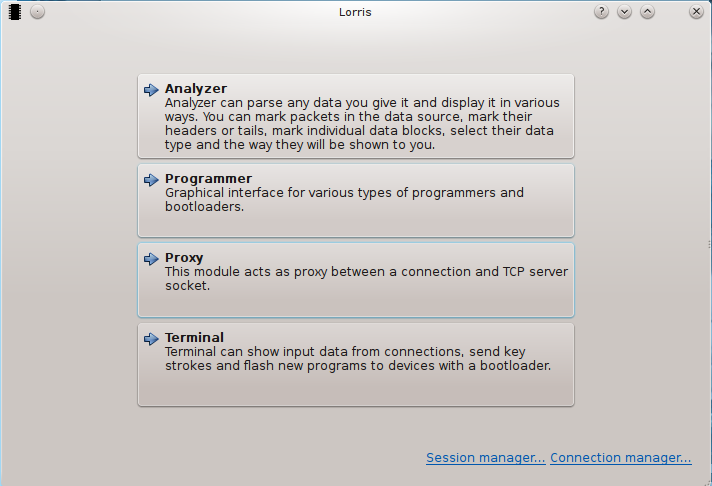
\includegraphics[scale=0.6]{img/new_tab.png}
\caption{Dialog vytvoření panelu}
\end{center}
\end{figure}

\begin{figure}[H]
\begin{center}
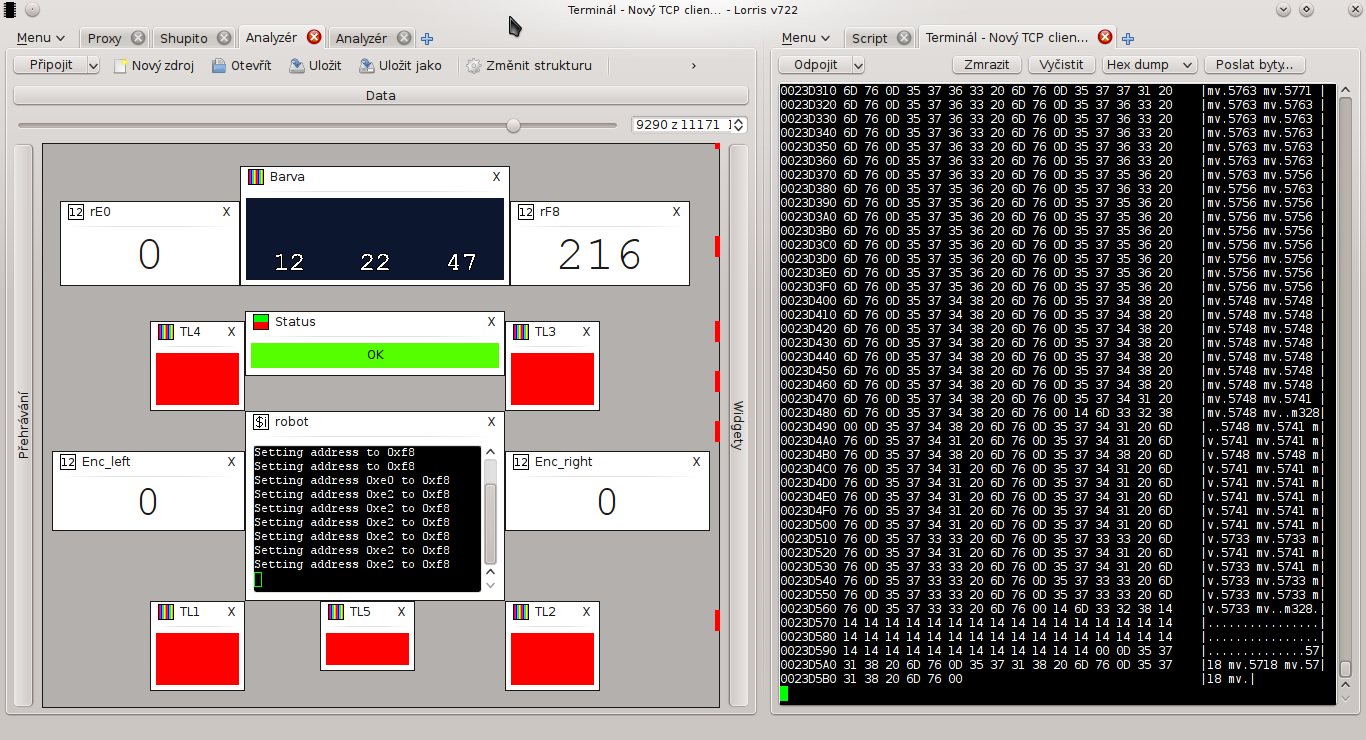
\includegraphics[width=\textwidth]{img/split.png}
\caption{Ukázka rozdělení okna na více částí}
\label{split_img}
\end{center}
\end{figure}

\subsection{Sezení}
Lorris dokáže uložit vše, co má uživatel aktuálně otevřené (záložky, jejich uspořádání, informace o připojení, data jednotlivých záložek atd.), jako tzv. sezení (anglicky \It{session}). Sezení je možné později načíst a tímto se vrátit k předchozí práci. Lorris automaticky ukládá sezení před svým ukončením, takže když uživatel program znovu otevře, vše je ve stejném stavu jako když aplikaci opouštěl.

\subsection{Automatická aktualizace}
Lorris se pod Windows dokáže sama aktualizovat. Při spuštění kontroluje zda je dostupná nová verze a pokud ano, zobrazí uživateli malé upozornění:
\begin{figure}[H]
\begin{center}

\includegraphics[scale=1]{img/update_notify.png}
\caption{Upozornění o dostupné aktualizaci}
\end{center}
\end{figure}
V případě, že uživatel aktualizaci potvrdí, se Lorris ukončí a spustí se malý pomocný program, který stáhne novou verzi a nainstaluje ji. Zobrazuje při tom seznam změn oproti staré verzi.
\begin{figure}[H]
\begin{center}
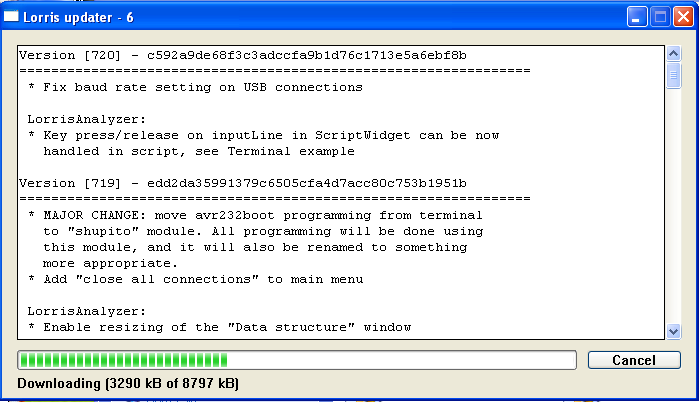
\includegraphics[width=\textwidth]{img/updater.png}
\caption{Probíhající aktualizace}
\end{center}
\end{figure}

\newpage
\section{Modul: Analyzér}

\begin{figure}[h]
\begin{center}
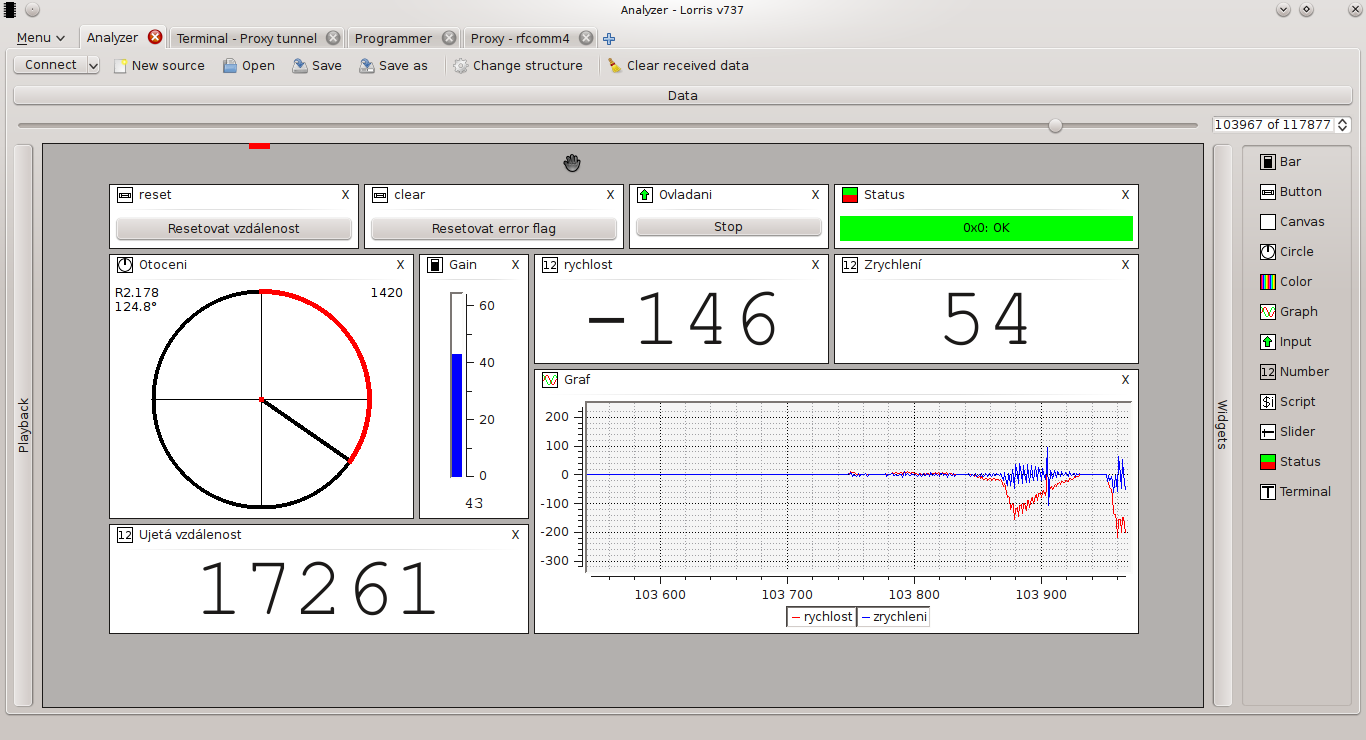
\includegraphics[width=\textwidth]{img/analyzer_all.png}
\caption{Modul analyzér}
\label{Analyzer}
\end{center}
\end{figure}

Tento modul parsuje data (strukturované do packetů) přicházející ze zařízení a zobrazuje je v grafických \uv{widgetech}. Zpracovaná data si aplikace ukládá do paměti -- listování packety je možné pomocí posuvníku a boxu v horní části okna. Data (přijatá data, struktura packetů a rozestavení a nastavení widgetů) je také možné uložit do souboru a později zase v programu otevřít.

Struktura dat se nastavuje v samostatném dialogu (viz obrázek \ref{Analyzer_struct}), kde je možno nastavit délku packetu, jeho endianness\footnote{\It{Endianness} -- pořadí uložení bajtů v paměti počítače}, přitomnost hlavičky a její obsah -- statická data (\uv{start bajt}), délka packetu (pokud je proměnná), příkaz a ID zařízení. Podle příkazu a ID zařízení je možno později data filtrovat.

\newpage
\setlength{\voffset}{0mm} % posune text/obrázek na této stránce, kam patøí
\pagestyle{plain}

Po nastavení struktury se přijatá data začnou po packetech zobrazovat v horní části okna, a v pravé části se zobrazí sloupeček s dostupnými zobrazovacími widgety. Widgety se dají pomocí drag\&drop principu \uv{vytahat} na plochu v prostřední části okna. Data se k widgetu přiřadí taktéž pomocí drag\&drop, tentokrát přetažení prvního bajtu dat na widget. 

Poté widget zobrazuje data tohoto bajtu, nebo tento bajt bere jako první, pokud jsou data delší. Aby bylo možné zpětně poznat, který bajt je k widgetu přiřazen, je po najetí myši na widget červeně zvýrazněn.

Nastavení widgetu jsou přistupná v kontextovém menu po pravém kliknutí myší na widget. Nastavit lze jméno a další parametry podle typu widgetu -- podrobněji jsou možnosti nastavení popsány u jednotlivých widgetů. Widgety je taktéž možné \uv{uzamknout}, aby nebylo možné je zavřít, měnit jejich pozici a velikost.

Widgety je možné přesně rozmisťovat pomocí \uv{přichytávání} k síti anebo k ostatním widgetům pomocí zarovnávacích čar (viz obrázek \ref{widget_lines}). Lze je také jednoduše a rychle duplikovat -- stačí přemístit widget se stiknutou klávesou control.

U některých widgetů se může hodit následující funkce: widgety je možné rychle zvětšit tak, aby zabraly celou viditelnou plochu pomocí gesta myší--stačí widget chytit jako při přesouvání a \uv{zatřepat} s ním zleva doprava. Při přesunutí se pak widget změnší na svoji původní velikost.

\begin{figure}[H]
\begin{center}
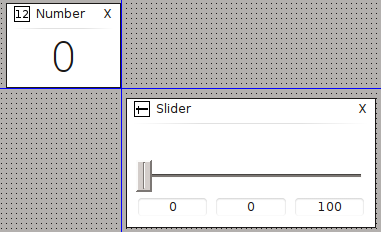
\includegraphics[scale=1]{img/lines.png}
\caption{Zarovnávání widgetů pomocí sítě a čar}
\label{widget_lines}
\end{center}
\end{figure}

\begin{figure}[H]
\begin{center}
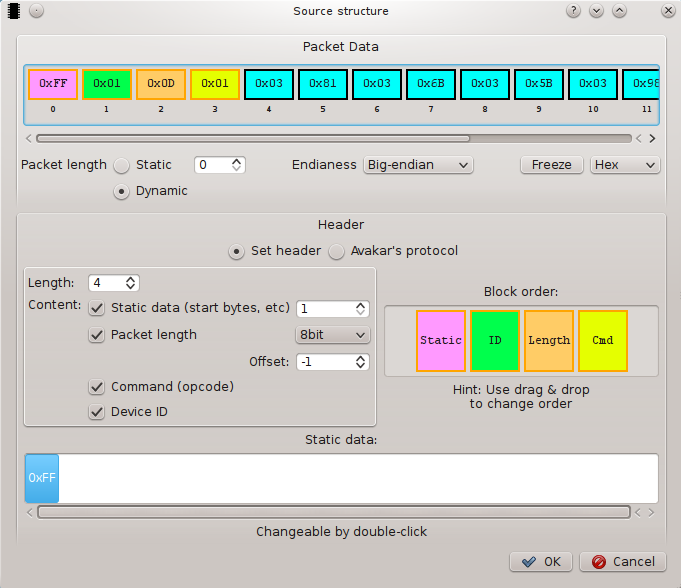
\includegraphics[scale=0.65]{img/analyzer_struct.png}
\caption{Dialog nastavení struktury dat}
\label{Analyzer_struct}
\end{center}
\end{figure}

\begin{figure}[H]
\begin{center}
\subfloat[Seznam widgetů]{\label{analyzer_widgets}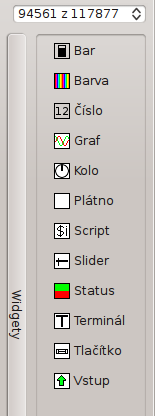
\includegraphics[scale=1]{img/analyzer_widgets_new.png}}
\hfill
\subfloat[Přiřazení dat pomocí drag\&drop]{\label{analyzer_widgets}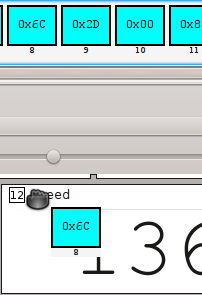
\includegraphics[scale=1]{img/analyzer_drag_data.png}}  
\caption{Widgety}
\label{widgets}
\end{center}
\end{figure}

\subsection{Filtrování dat}
Analyzér umí příchozí data filtrovat, přičemž každý filtr může obsahovat několik podmínek podle kterých se určí, zda příchozí packet projde nebo ne.
\begin{figure}[H]
\begin{center}
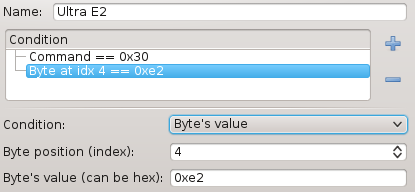
\includegraphics[scale=1]{img/filters.png}
\caption{Nastavení filtrů}
\end{center}
\end{figure}
Podmínka může kontrolovat buďto příkaz nebo zařízení z hlavičky packetu, hodnotu bajtu v packetu nebo může spustit jednoduchý uživatelský script. Díky scriptu je možné napsat takřka jakoukoliv podmínku pro filtrování.

\begin{listing}[H]
\begin{jscode}
// Vraci true pokud ma projit, false pokud ne
function dataPass(data, dev, cmd) {
    return false;
}
\end{jscode}
\caption{Script pro podmínku filtru}
\end{listing}

% TODO: newpage
\subsection{Widget: číslo}
\begin{figure}[h]
\begin{center}
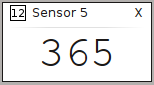
\includegraphics[scale=1]{img/w_num.png}
\caption{Widget: číslo}
\end{center}
\end{figure}
Tento widget dokáže zobrazovat celá čísla (se znaménkem i bez, 8 až 64 bitů dlouhé) a desetinná čisla (single-precision\footnote{Standardní formát uložení desetinných čísel v jazyku C a dalších (standard IEEE 754-2008).}, 32bit a 64bit).\\
Widget dále dokáže zarovnat číslo na maximální délku jeho datového typu\\a~formátovat ho těmito způsoby:
\begin{itemize}
    \item Desítkový -- číslo v desítkové soustavě
    \item Desítkový s exponentem -- použije exponent pro zapsaní velkých čísel. Dostupné pouze pro desetinná čísla.
    \item Hexadecimální -- výpis v šestnáctkové soustavě. Dostupné pouze pro přirozená čísla. 
    \item Binární -- zobrazí číslo ve dvojkové soustavě.  Dostupné pouze pro přirozená čísla.
\end{itemize}

Další funkcí je přepočítávání hodnoty pomocí výrazu. Toto se hodí například u~infračervených senzorů vzdálenosti, kdy se hodnota, kterou na senzoru naměří AD převodník, musí přepočítat pomocí určité rovnice abychom dostali hodnotu v centimetrech. Výraz může vypadat například takto:
\begin{center}
\verb|2914/(%n+5)-1|
\end{center}
kde \verb|%n| je zástupná sekvence pro číslo, které by se jinak ve widgetu zobrazilo. Tento výraz je pro přepočítání vzdálenosti na centimetry podle hodnoty přečtené z infračerveného senzoru vzdálenosti Sharp GP2Y0A41.

\subsection{Widget: sloupcový bar}
\begin{figure}[H]
\begin{center}
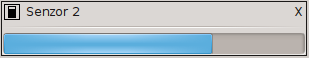
\includegraphics{img/w_bar.png}
\caption{Widget: sloupcový bar}
\end{center}
\end{figure}
Widget zobrazuje hodnotu ve sloupcovém baru. Lze nastavit datový typ vstupních dat (stejně jako u čísla), orientaci (vertikální nebo horizontální) a rozmezí zobrazovaných hodnot. Stejně jako widget číslo také dokáže přepočívat hodnotu podle výrazu.

\subsection{Widget: barva}
\begin{figure}[H]
\begin{center}
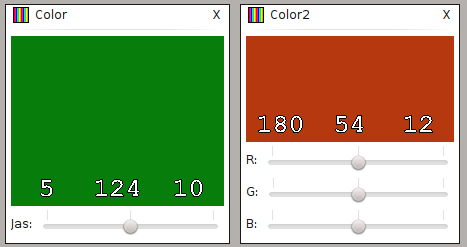
\includegraphics{img/w_col.png}
\caption{Widget: barva}
\end{center}
\end{figure}
Tento widget dokáže zobrazit příchozí hodnoty jako barevný obdélník. Podporované formáty:
\begin{itemize}
    \item {\bf RGB} (8b/kanál, 3x uint8)
    \item {\bf RGB} (10b/kanál, 3x uint16)
    \item {\bf RGB} (10b/kanál, 1x uint32)
    \item {\bf Odstíny šedé} (8b/kanál, 1x uint8)
    \item {\bf Odstíny šedé} (10b/kanál, 1x uint16)
\end{itemize}

Widget také dokáže provést korekci jasu všech barev zaráz nebo každé z barev RGB zvlášť.

\subsection{Widget: graf}
\begin{figure}[h]
\begin{center}
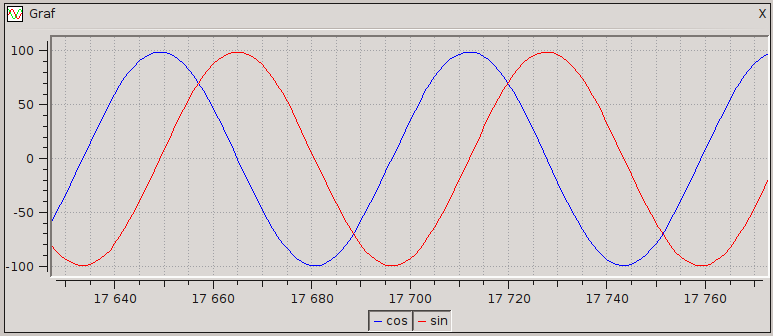
\includegraphics[scale=0.65]{img/w_graph.png}
\caption{Widget: graf}
\end{center}
\end{figure}
Widget graf zobrazuje hodnoty v grafu -- na osu $x$ se vynáší pořadí dat a na osu $y$ hodnoty dat. Lze nastavovat jméno, barvu a datový typ křivky grafu, automatické posouvání grafu, velikost vzorku, měřítko os grafu a zobrazení legendy. Kliknutí na křivku grafu v legendě tuto křivku skryje. Měřítko osy se ovládá otáčením kolečka myši po najetí kurzoru nad osu, po najetí do prostoru grafu se podobně ovládá měřítko celého grafu. 
\begin{figure}[h]
\begin{center}
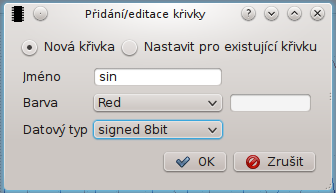
\includegraphics[scale=0.8]{img/w_graph_add.png}
\caption{Dialog pro nastavení parametrů křivky grafu}
\end{center}
\end{figure}

\subsection{Widget: script}
\begin{figure}[h]
\begin{center}
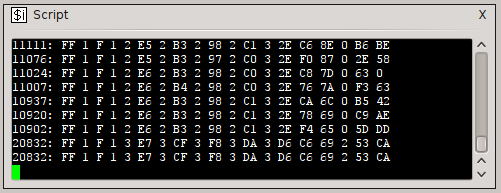
\includegraphics[scale=0.8]{img/w_script.png}
\caption{Widget: script}
\label{script_w}
\end{center}
\end{figure}
Tento widget umožňuje zpracovávání dat pomocí scriptu, který si napíše sám uživatel. Může při tom použít buďto Python nebo QtScript\cite{qtscript} (jazyk založený na standardu ECMAScript\footnote{\It{ECMAScript} -- scriptovací jazyk stadartu ECMA-262 a ISO/IEC 16262}, stejně jako JavaScript\footnote{\It{JavaScript} -- objektově orientovaný skriptovací jazyk, používaný hlavně na webu}, díky tomu jsou tyto jazyky velmi podobné). Script může zpracovávat příchozí data, reagovat na stisky kláves a posílat data do zařízení. Základní výstup může být zobrazen v terminálu (viz obrázek \ref{script_w}), je však možné využít ke zobrazování také ostatní widgety (číslo, bar, ...) -- script si je vytvoří jako objekt a nastavuje do nich data. Reference k vestavěným funkcím, které lze použít ve scriptu, je v \hyperref[script_ref]{příloze A}.

Editor scriptu má v sobě vestavěné ukázky kódu, například jak nastavit hodnotu existujícího widgetu \It{číslo}, jak odeslat data nebo jak reagovat na stisknutí klávesy (na obrázku \ref{script_src} jsou skryté pod ikonkou žárovky). Je v něm také odkaz na automaticky generovanou dokumentaci, která je na adrese \url{http://technika.junior.cz/docs/Lorris/}.
\begin{figure}[h]
\begin{center}
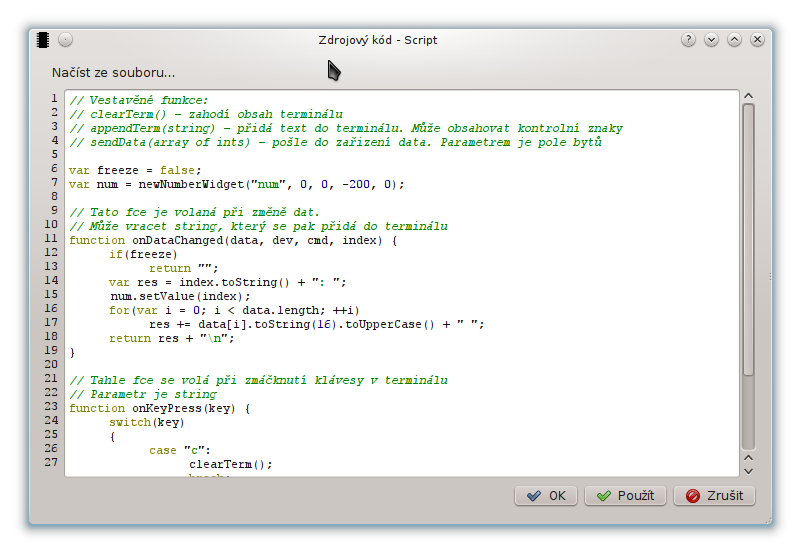
\includegraphics[width=\textwidth]{img/w_script_src.png}
\caption{Dialog pro nastavení zdrojového scriptu}
\label{script_src}
\end{center}
\end{figure}

\subsection{Widget: kolo}
\begin{figure}[H]
\begin{center}
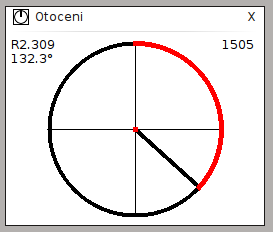
\includegraphics[scale=0.8]{img/w_circle.png}
\caption{Widget: kolo}
\end{center}
\end{figure}
Widget kolo zobrazuje příchozí hodnotu jako úhel v kruhu, což se hodí například při zobrazování natočení kola robota. Dokáže zobrazit data přicházející jako úhel ve stupních, radiánech nebo jako číslo v určitém rozmezí (například enkodér s rozlišením 12 bitů vrací číslo od 0 do 4095).

\subsection{Widget: plátno}
\begin{figure}[H]
\begin{center}
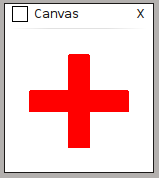
\includegraphics[scale=1]{img/w_canvas.png}
\caption{Widget: plátno}
\end{center}
\end{figure}
Plátno je widget který lze ovládat pouze ze scriptu a je určen ke kreslení 2D grafiky. Dokáže zobrazit čáry, obdélníky, kruhy a elipsy. V následujícím příkladu je kód pro nakreslení červeného kříže uprosřed widgetu.

\begin{listing}[H]
\begin{jscode}
Canvas.setLineColor("red");
Canvas.setFillColor("red");
// x, y, sirka, vyska
Canvas.drawRect(55, 10, 20, 110);
Canvas.drawRect(10, 55, 110, 20);
\end{jscode}
\caption{Ovládání widgetu plátno}
\end{listing}

\subsection{Widgety tlačítko a slider}
\begin{figure}[H]
\begin{center}
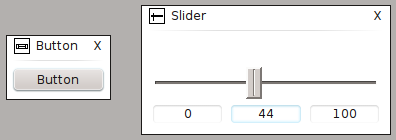
\includegraphics[scale=1]{img/w_btn_slider.png}
\caption{Widgety tlačítko a slider}
\end{center}
\end{figure}
Tyto dva widgety pouze umožňují interakci se scriptem -- po stisknutí tlačítka se zavolá metoda ve scriptu, ve které může uživatel například poslat příkaz do robota, při posunutí slideru se ve scriptu zavolá metoda, ve které může uživatel například změnit rychlost robota a podobně. Tlačítku lze nastavit klávesovou zkratku a slideru zkratku pro \uv{zaostření}, aby ho uživatel poté mohl posouvat pomocí šipek na klávesnici.
\begin{listing}[H]
\begin{jscode}
function Slider_valueChanged() {
    appendTerm("Hodnota slideru " + Slider.getValue() + "\n");
}

function Tlacitko_clicked() {
    appendTerm("Tlacitko stisknuto\n");
}
\end{jscode}
\caption{Metody volané widgety \It{slider} a \It{tlačítko}}
\end{listing}

\subsection{Widget: vstup}
\begin{figure}[H]
\begin{center}
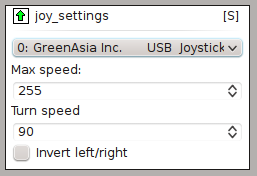
\includegraphics[scale=1]{img/w_input.png}
\caption{Widget \It{vstup} s nastavením joysticku}
\label{input}
\end{center}
\end{figure}
Tento widget je také určený k interakci se scriptem (tj. vstupu uživatele), přičemž script také určuje prvky rozhraní -- widget je v základu prázdný a až script do něj přidá například tlačítko nebo textové pole. Tento widget je mírně složitější na obsluhu, ale lze díky němu použít všechny prvky UI, které Qt Framework obsahuje -- tlačítka, posuvníky, textová pole, vysouvací seznamy a podobně. V příkladu \ref{input_script} je script pro vytvoření prvků jako v obrázku \ref{input}.

\begin{listing}[H]
\begin{jscode}
// parametry: jmeno Qt widgetu, "stretch" hodnota
var joyList = joy_settings.newWidget("QComboBox");
var maxSpdLabel = joy_settings.newWidget("QLabel", 1);
var maxSpd = joy_settings.newWidget("QSpinBox");
var turnSpdLabel = joy_settings.newWidget("QLabel", 1);
var turnSpd = joy_settings.newWidget("QSpinBox");
var invert = input.newWidget("QCheckBox");

// Nastaveni textu do QLabel
maxSpdLabel.text = "Max speed:";
\end{jscode}
\caption{Přidání prvků do widgetu \It{vstup}}
\label{input_script}
\end{listing}

\subsection{Widget: status}
\begin{figure}[H]
\begin{center}
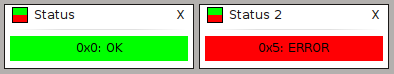
\includegraphics[scale=1]{img/w_status.png}
\caption{Widget status}
\end{center}
\end{figure}
Widget status je určený k zobrazování stavu například tlačítka (stisknuté/nestisknuté) nebo chybového stavu z enkodéru (0 = vše je v pořádku, ostatní čísla je možné dohledat v datasheetu enkodéru). Uživatel k příchozím hodnotám přiřadí jednotlivé stavy (text a barvu, viz obrázek \ref{status_dlg}) a widget je poté zobrazuje. Lze nastavit i \uv{neznámou hodnotu}, která se zobrazí pokud žádný z nadefinovaných stavů neodpovídá příchozí hodnotě.
\begin{figure}[H]
\begin{center}
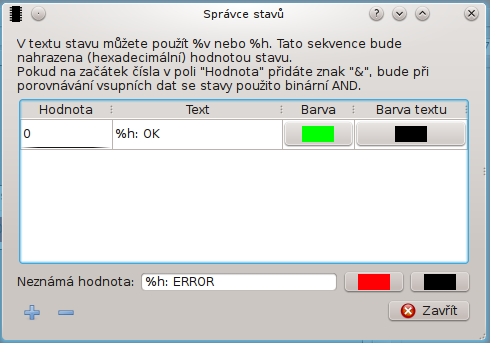
\includegraphics[scale=1]{img/w_status_dlg.png}
\caption{Nastavení stavů}
\label{status_dlg}
\end{center}
\end{figure} 

\subsection{Widget: terminál}
\begin{figure}[H]
\begin{center}
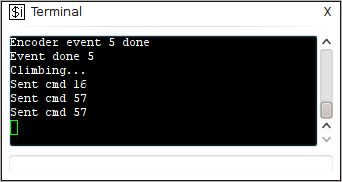
\includegraphics[scale=0.70]{img/w_terminal.png}
\caption{Widget terminál}
\end{center}
\end{figure}
Tento widget je zde pouze pro pohodlí uživatele, jedná se totiž o widget \It{script} ve kterém je přednastavený kód díky kterému se widget chová stejně jako terminál. Uživatel může script tohoto widgetu libovolně upravovat.

\newpage
\setlength{\voffset}{0mm} % posune text/obrázek na této stránce, kam patøí
\pagestyle{plain}
\section{Modul: Proxy mezi sériovým portem a TCP socketem}
\begin{figure}[H]
\begin{center}
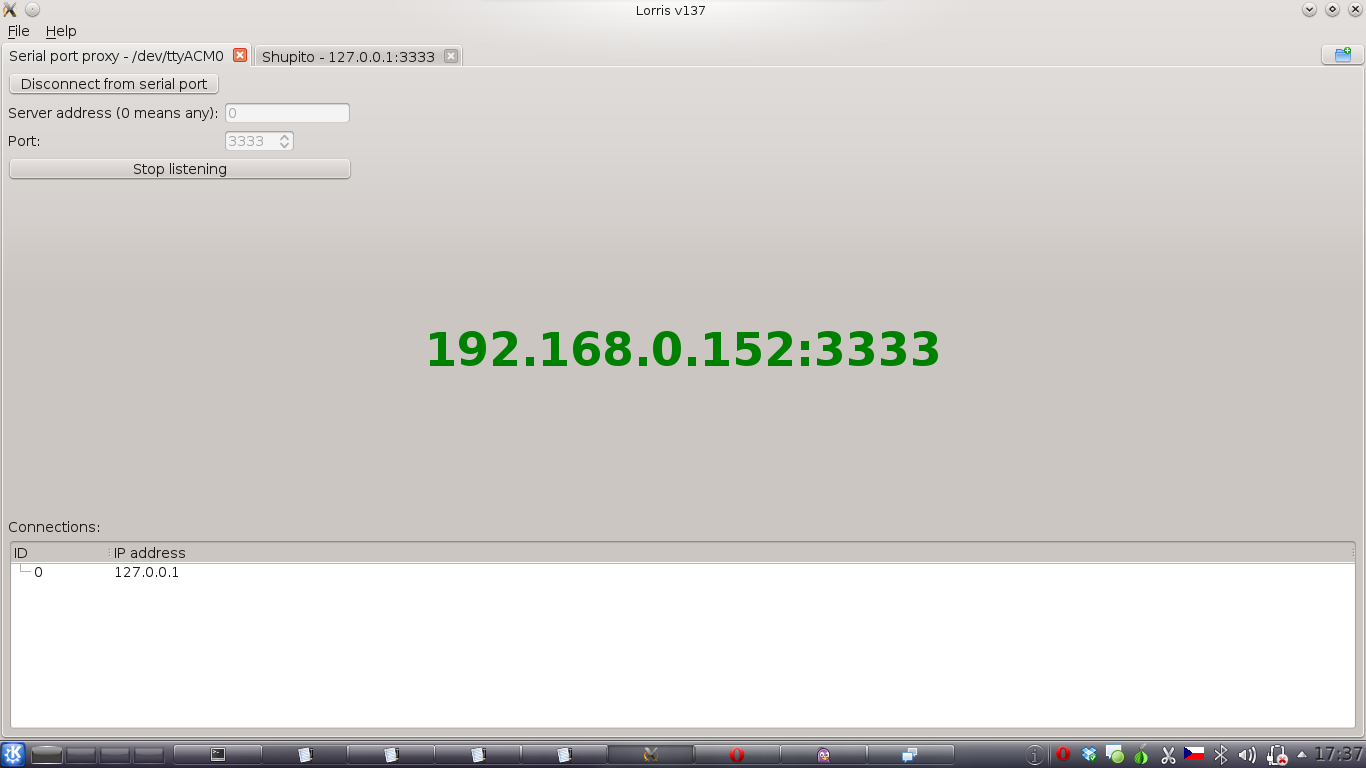
\includegraphics[width=\textwidth]{img/proxy.png}
\caption{Proxy mezi sériovým portem a TCP socketem}
\label{Shupito}
\end{center}
\end{figure}
Jednoduchá proxy mezi sériovým portem a TCP socketem. Vytvoří server, na který je možné se připojit z Lorris nebo jiného programu na jiném počítači. Po připojení se přeposílají data ze sériového portu připojeným klientům a naopak.

\subsection{Proxy tunel}
Tento modul také přidává nové virtuální připojení - \uv{proxy tunel}. Pokud toto připojení použije nějáký z dalších modulů v Lorris, tak může posílat a přijímat data od všech TCP klientů připojených na proxy. Toto je možné využít například tak, že v modulu analyzér je script, který generuje data a přes proxy tunel je pak odesílá všem klientům připojeným na proxy.

\newpage
\setlength{\voffset}{0mm} % posune text/obrázek na této stránce, kam patøí
\pagestyle{plain}

\section{Modul: Programátor}
\begin{figure}[H]
\begin{center}
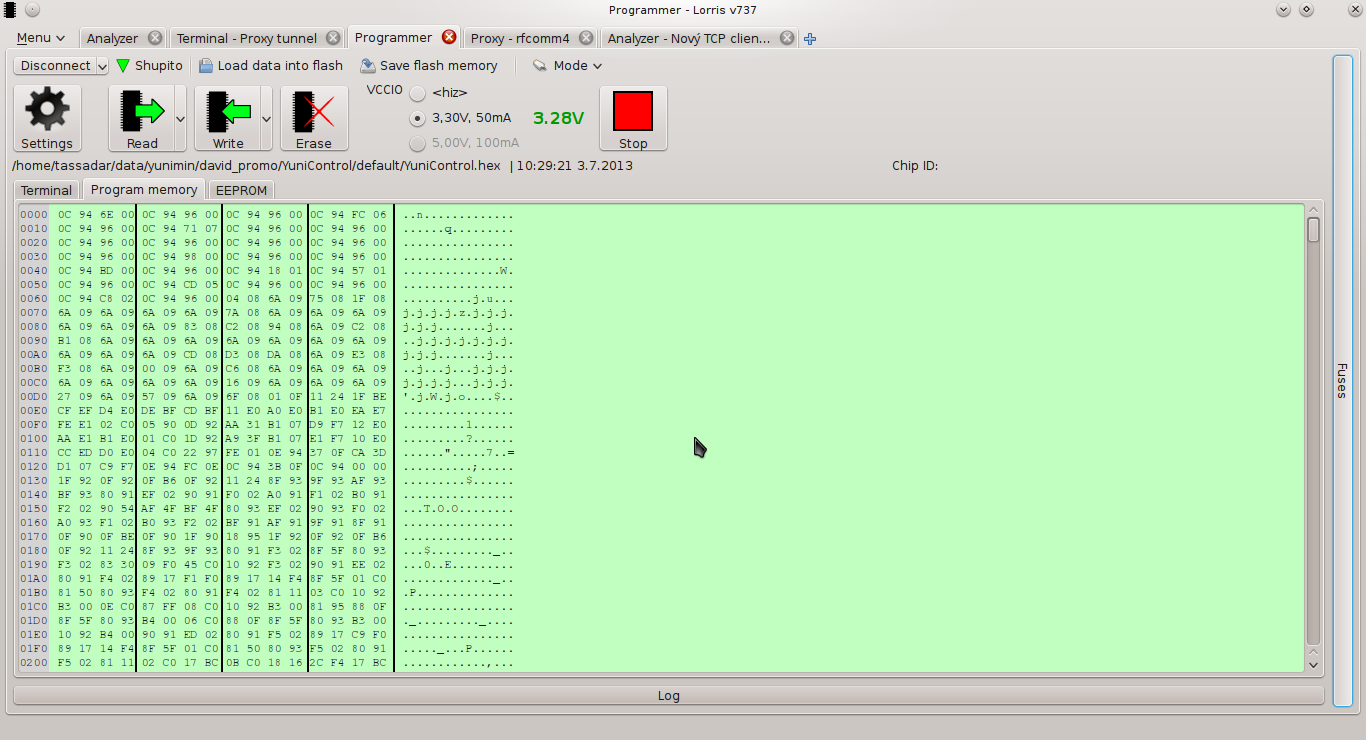
\includegraphics[width=\textwidth]{img/programmer.png}
\caption{Modul Programátor}
\label{prog_full}
\end{center}
\end{figure}

%TODO: rozšířit
Tento modul funguje jako grafické rozhraní pro několik typů programátorů a bootloaderů. Podporuje dva typy rozhraní -- plné (obrázek \ref{prog_full}) a zmenšené (obrázek \ref{prog_mini}). Plné rozhraní obsahuje tlačítka a nastavení pro programování všech pamětí čipu, zmenšené rozhraní pak obsahuje pouze tlačítko na programování hlavní paměti a zastavení čipu. Zmenšený mód je vhodný při rozdělení okna na více částí protože obsahuje pouze nejpoužívanější prvky a nezabírá zbytečně místo.

\begin{figure}[H]
\begin{center}
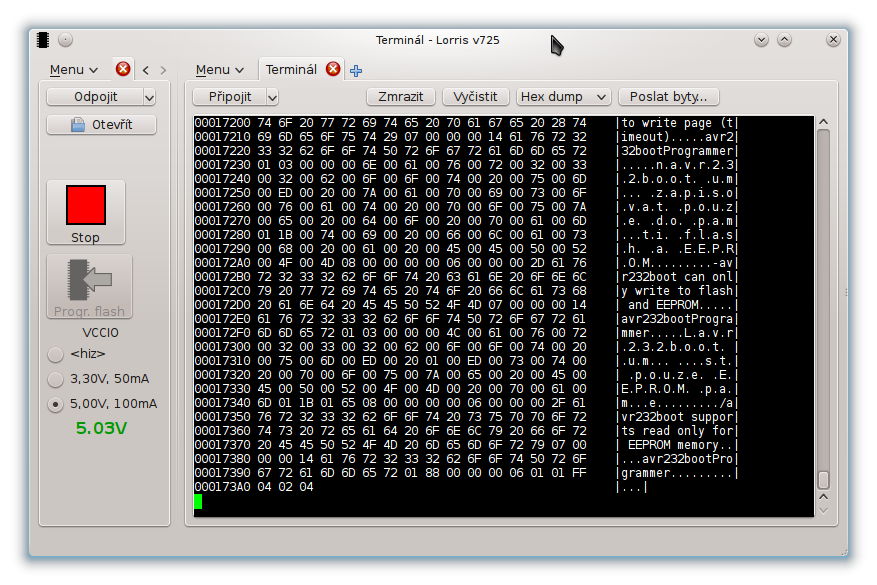
\includegraphics[width=\textwidth]{img/programmer_mini.png}
\caption{Zmenšené UI modulu \It{programátor} (nalevo) s otevřeným \It{terminálem}}
\label{prog_mini}
\end{center}
\end{figure}

\subsection{Programátor Shupito}
Shupito je programátor mikročipů vytvořený Martinem Vejnárem, který dokáže programovat mikrokontroléry pomocí ISP\footnote{\It{In-system programming} -- rozhraní, které umožňuje programovat čipy přímo na desce plošného spoje.}, PDI\footnote{\It{Program and Debug Interface} -- rozhraní firmy Atmel umožňující programování čipů přímo na desce, podobně jako ISP} a JTAG\footnote{\It{Joint Test Action Group} -- rozhraní podle standardu IEEE 1149.1 umožňující mimo jiné programování a debugování čipů} rozhraní. 

Modul programátor v mojí práci slouží jako oficiální rozhraní pro Shupito. Převážná část komunikace s programátor je napsána samotným Martinem Vejnárem.

\subsubsection{UART tunel}
\label{tunel}
Shupito dokáže vytvořit tunel\footnote{Přímé spojení programovaného čipu a počítače přes programátor.} pro UART linku z programovaného čipu do počítače. Lorris umí této funkce využít -- aktivní tunel se zobrazí jako další typ připojení a je možné se na něj připojit v ostatních modulech.


\begin{figure}[H]
\begin{center}
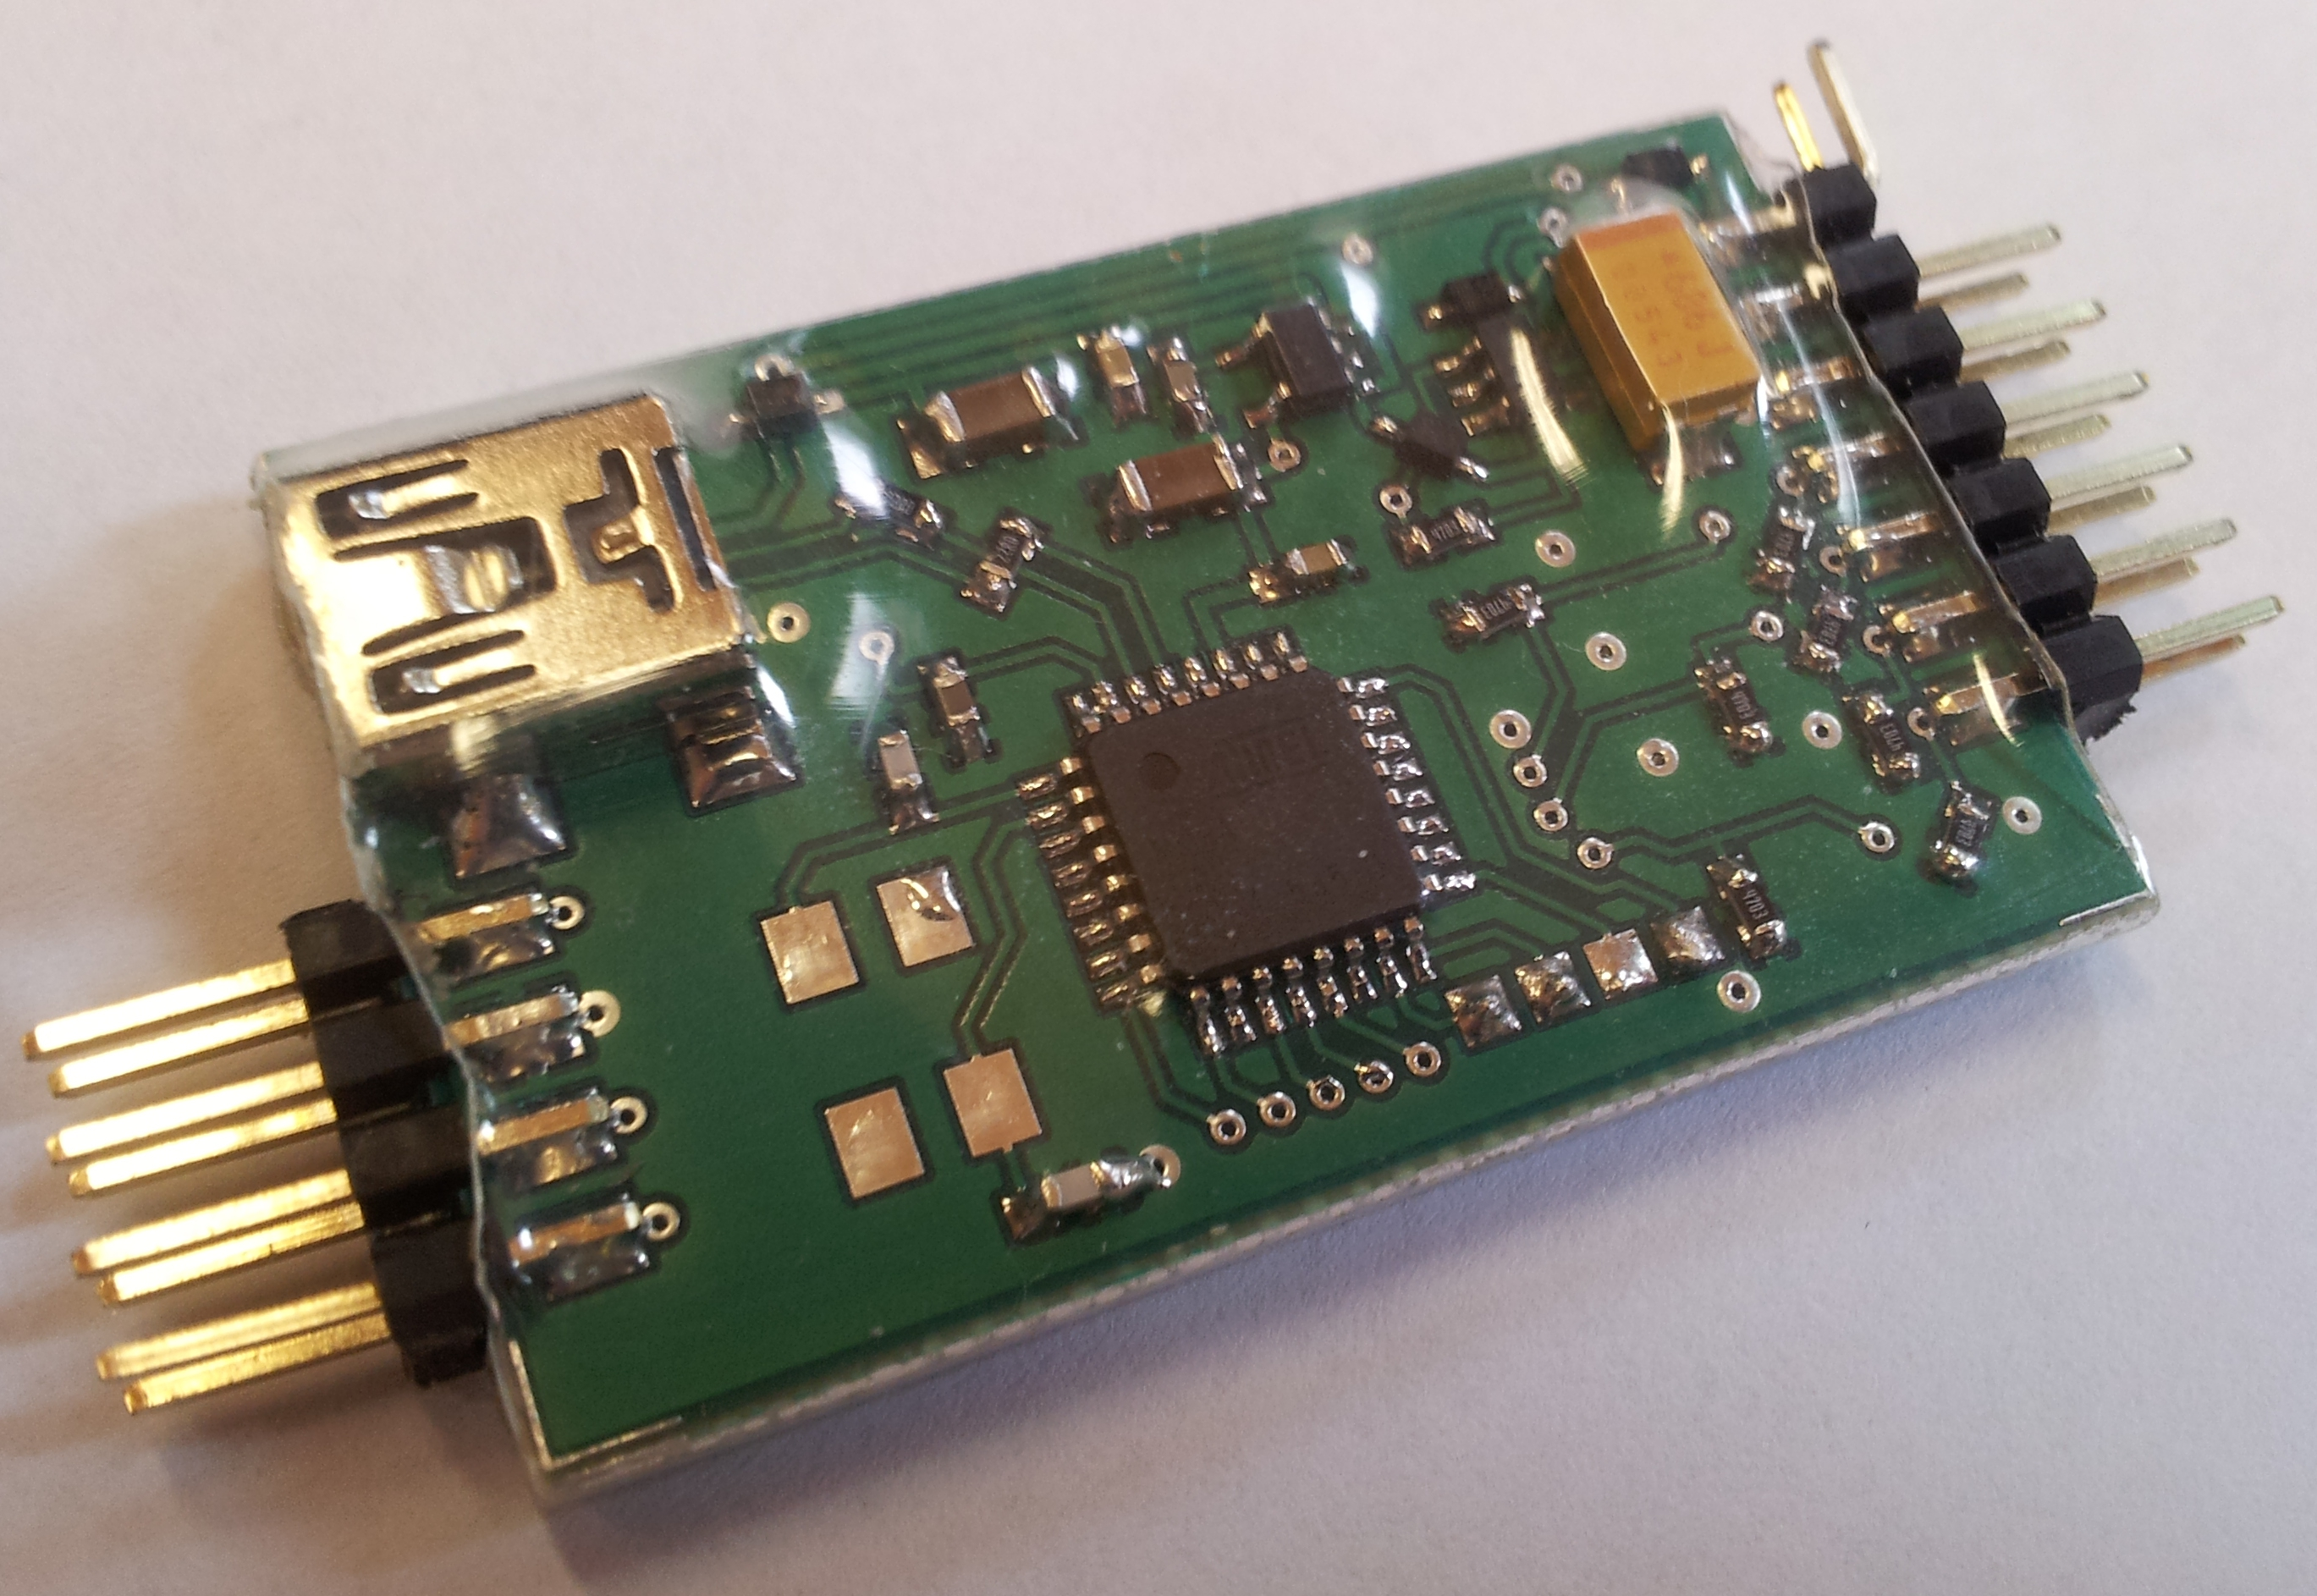
\includegraphics[width=\textwidth]{img/shupito_promo.jpg}
\caption{Programátor \It{Shupito}}
\label{prog_mini}
\end{center}
\end{figure}

\subsection{Bootloader avr232boot}
Autorem tohoto bootloaderu je také Martin Vejnár. Avr232boot je pouze pro čipy Atmel ATmega a je inspirovaný referenčním bootloaderem pro tyto mikrokontroléry, je však napsaný tak, aby zabíral v čipu co nejméně místa. Původně uměl pouze programovat flash paměť čipu (ta, ve které je uložen program), já jsem do něj přidal podporu čtení a zapisování paměti EEPROM\footnote{Typ paměti, která udrží data i bez proudu. V čipech se používá na uložení např. nastavení}.

Lorris dokáže pomocí tohoto bootloaderu programovat flash paměť a číst a programovat EEPROM.

\subsection{Bootloader AVROSP}
\It{AVR Open Source Programmer} je protokol používaný několika bootloadery firmy Atmel pro čipy ATmega a ATxmega. Lorris dokáže pomocí toho bootloaderu programovat a číst flash i EEPROM paměť čipu.


\newpage
\section{Modul: Terminál}
\begin{figure}[H]
\begin{center}
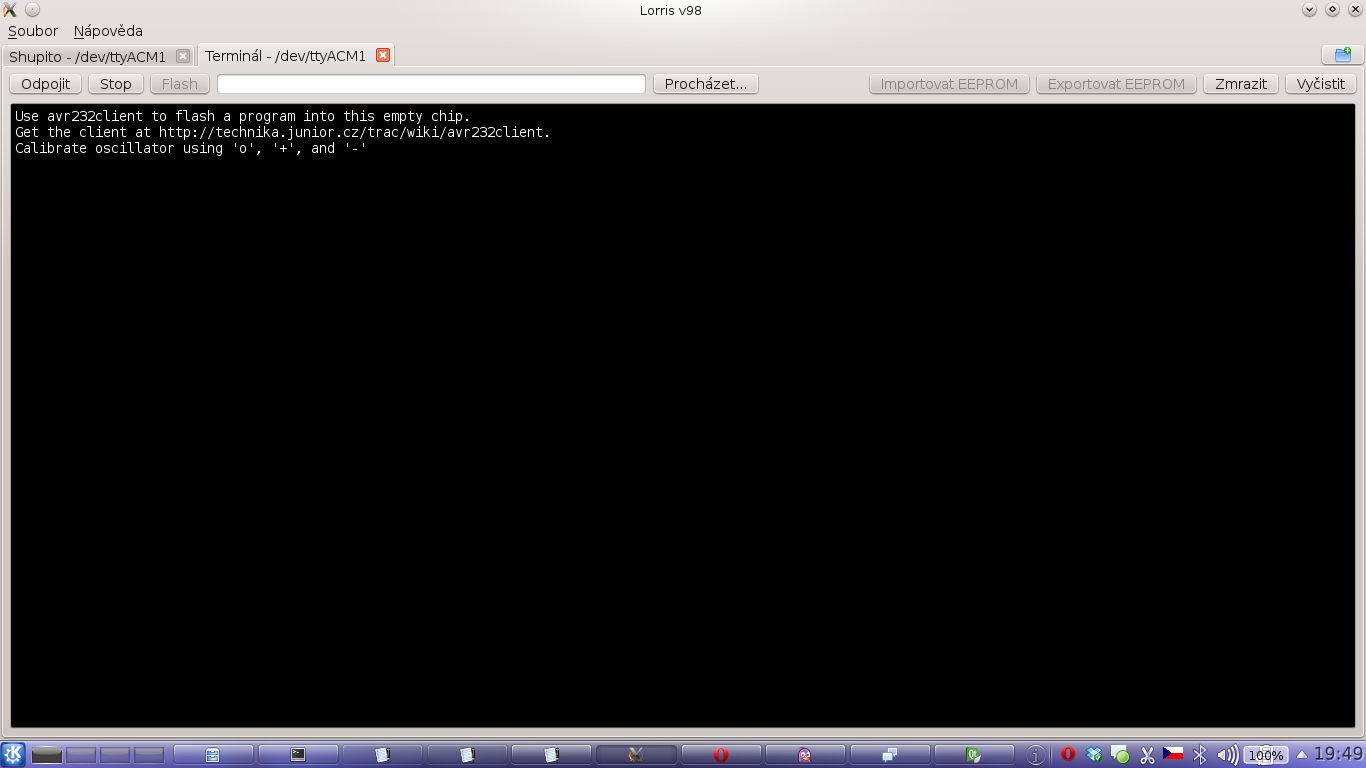
\includegraphics[width=\textwidth]{img/terminal.png}
\caption{Modul terminál}
\label{Terminal}
\end{center}
\end{figure}
Základní pomůcka při práci s mikrokontroléry, běžný textový -- zobrazuje data přijatá přes sériový port a posílá stisky kláves. Kromě klasického textového módu dokáže příchozí data zobrazovat jako hexadecimální hodnoty všech příchozích bajtů.

Terminálu je možné nastavit barevné schéma, velikost a font textu, jaká sekvence kontrolních znaků se má odeslat při stisknutí klávesy enter a chování některých kontrolních znaků (například jestli má znak \verb|\n| vytvořit nový řádek nebo ne).

\newpage
\section{Podpora joysticku}
Lorris podporuje použití joysticku v modulu analyzér například k řízení robota. Nejdříve jsem k přístupu k joysticku používal knihovnu SDL\cite{sdl}, ta však pro moje použití nebyla příliš vhodná -- tuto knihovnu autoři vytvořili jako základ pro tvorbu počítačových her a podpora joysticku je tedy jen jedna z mnoha částí, které knihovna obsahuje. Její architektura se také nehodila ke zbytku Lorris.

Při hledání náhrady jsem ale nenašel žádnou vhodnou knihovnu, jejíž funkce by byla pouze přistupování k joysticku a neměla žádné zbytečné funkce které bych v Lorris nepoužil, a tak jsem si napsal vlastní knihovnu.

Jmenuje se {\bf libenjoy}, funguje pod Windows a Linuxem a je velmi malá a jednoduchá. Oproti SDL si dokáže zapamatovat připojené joysticky, a když joystick odpojíte a zase ho připojíte zpět (například kvůli přeskládání kabelů u počítače nebo se joystick odpojí sám kvůli špatnému kontaktu), není třeba ho znovu vybírat jako aktivní, sám se připojí bez jakékoliv interakce uživatele.

Libenjoy je vydána pod licencí GNU LGPLv2.1\cite{lgpl}.

\begin{itemize}
\item GIT repozitář: \url{https://github.com/Tasssadar/libenjoy}
\end{itemize}

\newpage
\section{Příklady použití}
\subsection{Testování barevného senzoru}
{\bf Situace:} Stavím robota do soutěže (Eurobot, RobotChallange, ...), ve které je možné se na herním poli orientovat podle barvy. Chci barevný senzor otestovat, proto jsem na nepájivém poli postavil jednoduchý obvod s čipem, na který je senzor připojený. Čip bude dávat senzoru pokyny k měření a vyčítat z něj RGB hodnoty, které následně pošle do RS232 linky.\\
\\
{\bf Řešení:} Program, který bude ze senzoru číst hodnoty naprogramuji do čipu pomocí programátoru Shupito, který také poskytne tunel pro RS232 linku. Na tento tunel se připojím modulem Analyzér, ve kterém díky widgetu \uv{barva} mohu vidět barvu, kterou senzor rozpoznal.

\begin{figure}[h]
\begin{center}
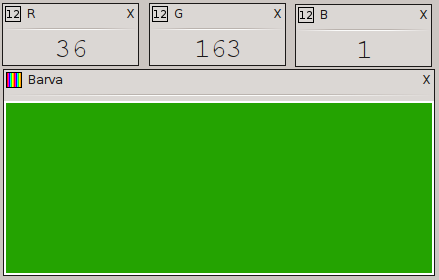
\includegraphics{img/use_color.png}
\caption{Barva v modulu Analyzér}
\end{center}
\end{figure}

\newpage
\subsection{Testování enkodéru}
V roce 2012 vypracoval můj spolužák Marek Ortcikr práci SOČ \It{Modulární stavba robota} ve které byl jedním z modulů magnetický vlečný enkodér. Tento modul vypadá jako další kolečko, které se na robota připevní, uvniř osy kola je však magnet a naproti němu napevno uchycený čip enkodéru. Čip snímá orientaci magnetického pole vytvořeného magnetem v ose kola a~podle toho dokáže určit jeho natočení. Enkodér poté sleduje změny v natočení kola podle kterých je možné zjistit ujetou vzdálenost, rychlost a zrychlení robota.
\begin{figure}[H]
\begin{center}
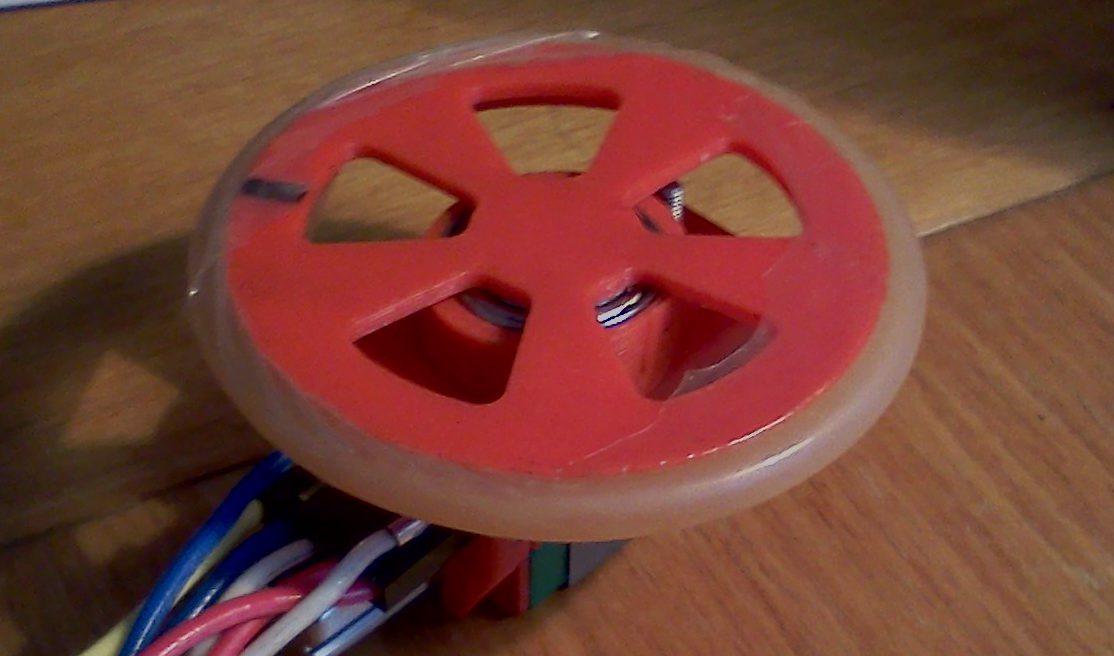
\includegraphics[width=\textwidth]{img/enc_real.png}
\caption{Magnetický enkodér}
\end{center}
\end{figure}
Pro demonstraci enkodéru na celostatním kole soutěže SOČ byla použita moje aplikace Lorris. Celé rozhraní je vidět na obrázku \ref{analyzer_all} na straně \pageref{analyzer_all}, zde jsou popsány jednotlivé části zvlášť.

\begin{figure}[H]
\begin{center}
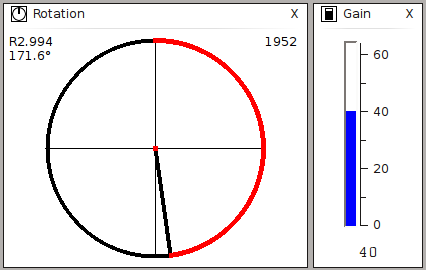
\includegraphics[width=\textwidth-45pt]{img/enc_circle.png}
\caption{Natočení kola}
\end{center}
\end{figure}
Widget \It{kolo} zde znázorňuje aktuální natočení kolečka enkodéru. V pravém horním rohu je aktuální hodnota z enkodéru (0 až 4095), vlevo je hodnota přepočítaná na radiány a stupně.

Widget \It{bar} pojmenovaný \uv{gain} ukazuje sílu magnetického pole, tedy jak daleko je magnet v ose kolečka od čipu enkodéru. Hodnota má rozmezí od 0 do 63, ideální je zhruba střed tohoto rozmezí.

\begin{figure}[H]
\begin{center}
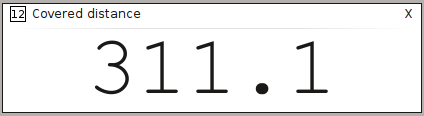
\includegraphics[scale=0.85]{img/enc_dist.png}
\caption{Ujetá vzdálenost}
\end{center}
\end{figure}
Tento widget \It{číslo} zobrazuje naměřenou vzdálenost v milimetrech. Enkodér odesílá tuto informaci v $\frac{1}{4096}$ obvodu kolečka, takže je třeba ji přepočítat pomocí výrazu \verb|%n/32.5949|.

\begin{figure}[H]
\begin{center}
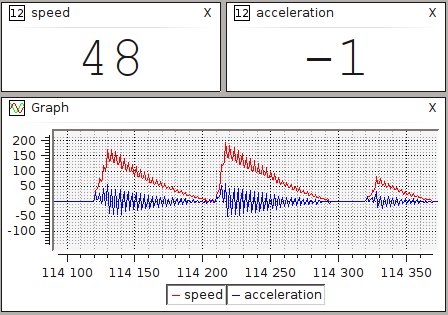
\includegraphics[width=\textwidth-60pt]{img/enc_spd.png}
\caption{Rychlost a zrychlení}
\end{center}
\end{figure}
Dva widgety \It{číslo} jsou zde použity k zobrazení aktuální rychlosti a zrychlení. Pod nimi je widget \It{graf} ve kterém je rychlost jako červená křivka a zrychlení jako modrá.

\begin{figure}[H]
\begin{center}
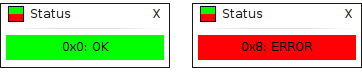
\includegraphics[width=\textwidth]{img/enc_status.png}
\caption{Stav enkodéru}
\end{center}
\end{figure}
Čip enkodéru také informuje o svém stavu, pokud je vše v pořádku vrací číslo \verb|0x0|, narazí-li na nějáký problém, vrátí některý z chybových kódů (například \verb|0x8| při nepřítomnosti magnetu v ose kola). Widget \It{status} ukazuje chybový kód a barvu podle informací z enkodéru.

\begin{figure}[H]
\begin{center}
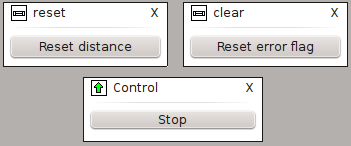
\includegraphics[width=\textwidth-50pt]{img/enc_ctrl.png}
\caption{Ovládání enkodéru}
\end{center}
\end{figure}
Tyto widget \It{tlačítko} a \It{vstup} obstarávají ovládání enkodéru. Tlačítko \uv{reset} vrátí počítadlo ujeté vzdálenosti na nulu, tlačítko \uv{clear} pošle enkodéru příkaz k resetu chybového kódu (kód po chybě zůstává i když příčina již byla napravena, je třeba ho resetovat) a tlačítko \uv{Ovladani} zastavuje a spouští posílání dat z enkodéru. Všechny tyto widgety jsou připojené na script (do obrázku \ref{analyzer_all} se už widget script nevešel), který po kliknutí na tlačíka odešle do enkodéru příslušné příkazy.
\begin{listing}[H]
\begin{jscode}
var run = true;
function reset_clicked() {
    sendData(new Array(0xFF, 0x01, 0x01, 0x00));
}
function clear_clicked() {
    sendData(new Array(0xFF, 0x01, 0x01, 0x01));
}
function startStop_clicked() {
    run = !run;
    startStopBtn.text = run ? "Stop" : "Start";
    sendData(new Array(0xFF, 0x01, 0x02, 0x02, run ? 1 : 0));
}
\end{jscode}
\caption{Script, který odesílá příkazy do enkodéru}
\end{listing}

\newpage
\subsection{Ladění PID regulátoru}
{\bf Situace:} Robot kvůli rozdílnému výkonu motorů nejede rovně. Tento problém jsem se rozhodl řešit pomocí PID regulátoru, pro jehož správnou funkci je potřeba nastavit několik konstant. \\
\\
{\bf Řešení:} Program v robotovi mi posílá aktualní výkon motorů a nastavení konstant PID regulátoru a umožňuje přenastavení těchto konstant a ovládání robota. Tento program do robota nahrávám přes bluetooth pomocí modulu Terminál, protože čip má v sobě bootloader -- díky tomu nemusím mít připojený programátor.  

V modulu analyzér si zobrazím aktuální hodnoty PID regulátoru (jako číslo) a výkon motorů (jako graf či číslo). Do widgetu script napíši jednoduchý script, který po stisku kláves změní nastavení konstant regulátoru nebo rozjede/zastaví robota.

Tento postup jsem použil při ladění PID regulátoru robota 3pi\cite{3pi} během přípravy na soutěž \It{Line Follower Standard}, která je součástí Robotického dne 2012\cite{rob_den}. Na soutěži jsem skončil na 2. místě z 22 robotů\cite{robotday_res}.
\begin{figure}[H]
\begin{center}
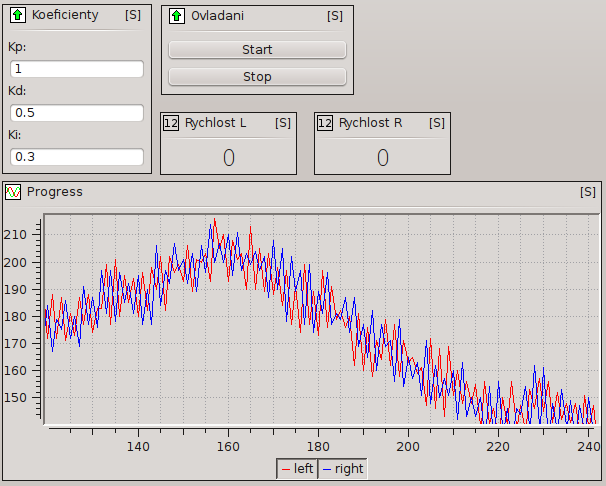
\includegraphics[scale=0.55]{img/use_pid.png}
\caption{Ladění PID regulátoru}
\end{center}
\end{figure}

\newpage
\subsection{Stavba robota pro soutěž Eurobot 2011}
Použití mého programu Lorris je zde prezentováno na příkladu stavby robota, který vznikal na naší škole (SPŠ a VOŠ technická, Sokolská 1, Brno) v roce 2011 pro soutěž Eurobot\cite{eurobot} (fotku robota najdete v přílohách na straně \pageref{david}, obrázek č. \ref{david}).

Ačkoliv je robot již 2 roky starý a celá sada Lorris se od té doby značně posunula vpřed, robot \It{David} představuje velmi dobrý příklad využití velké části funkcí celého balíku nástrojů.

Cíl soutěže je každý rok jiný, v roce 2011 měli roboti za úkol hrát něco jako zjednodušené šachy. Herní hřiště bylo rozděleno na barevnou šachovnici a leželi na něm \uv{pěšci} (žluté disky), které měli roboti posouvat na políčka svojí barvy, případně z nich stavět věže. Vyhrával robot s největším počtem bodů, které získával za pěšce na polích svojí barvy a postavené věže. Roboti navíc musí mít vyřešenou detekci soupeře, aby do sebe nenaráželi (např. pomocí ultrazvukových dálkoměrů). Kompletní pravidla, výsledková listina a další informace jsou na webu ročníku 2011\cite{eurobot11}.

Právě při vývoji tohoto robota vyvstala palčivá potřeba mít k dispozici nástroj, který by umožňoval ve všech fázích jeho vývoje snadné a rychlé testování a ladění všech funkcí a komponent robota. Vzhledem k tomu, že nejviditelnější částí programu Lorris je nástroj Analyzér, je v této ukázce prezentováno především jeho použití, ostatní nástroje (Programátor, Terminál) však byly také použity, například při programování mikročipu v robotovi.

V příkladu je vytvořeno jednoduché uživatelské prostředí pro ovládání, testování a programování pro jednoho robota. Toto prostředí však lze znovu použít i pro jiného robota anebo vytvořit nové, pokud je robot příliš atypický a vyžaduje jiný typ ovládání.


\newpage
\subsubsection{Mechanická kostra robota}
Jako první byla navržena mechanická konstrukce robota. Již v této fázi byla využita moje aplikace Lorris. Pro otestování funkčnosti a chování motorů a servomotorů bylo použito ovládání pomocí joysticku. V Lorris jsem sestavil menší skupinu widgetů: \It{Script}, který čte data z joysticku, přepočítává je na rychlosti, které je třeba nastavit motorům a odesílá je do robota. Dále widget \It{Vstup}, ve kterém je nastavení ovládání pomocí joysticku a 2 widgety \It{Číslo}, které zobrazují aktuální rychlosti motorů.
\vspace{30mm}
\begin{center}
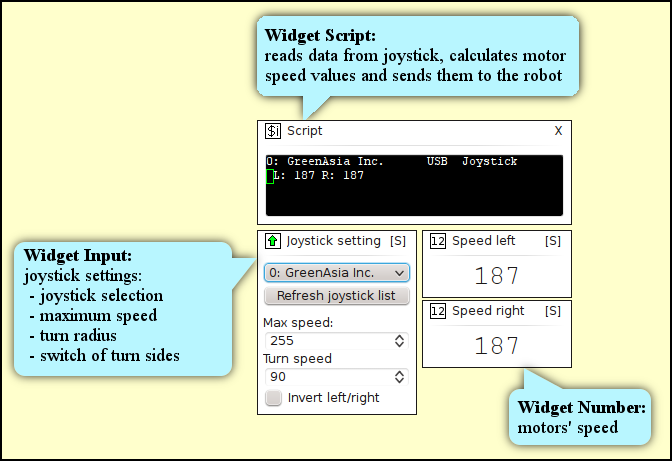
\includegraphics[width=\textwidth]{img/joystick_david.png}
\end{center}

\newpage
\subsubsection{Ladění a nastavení senzorů}
Po vyladění mechanické části robota byl osazen senzory. Po jejich umístění jsem v nástroji Analyzér vytvořil rozhraní, které využívá zejména widgetů \It{Script}, \It{Číslo}, \It{Barva} a \It{Status}. Každý z těchto widgetů je možné na pracovní ploše Analyzéru přesouvat, zmenšovat nebo zvětšovat, díky čemuž je možné jejich rozmístění tak, aby odpovídalo skutečným pozicím senzorů na robotu. Jako optimální se jeví zobrazení jako při pohledu shora.
\vspace{10mm}
\begin{center}
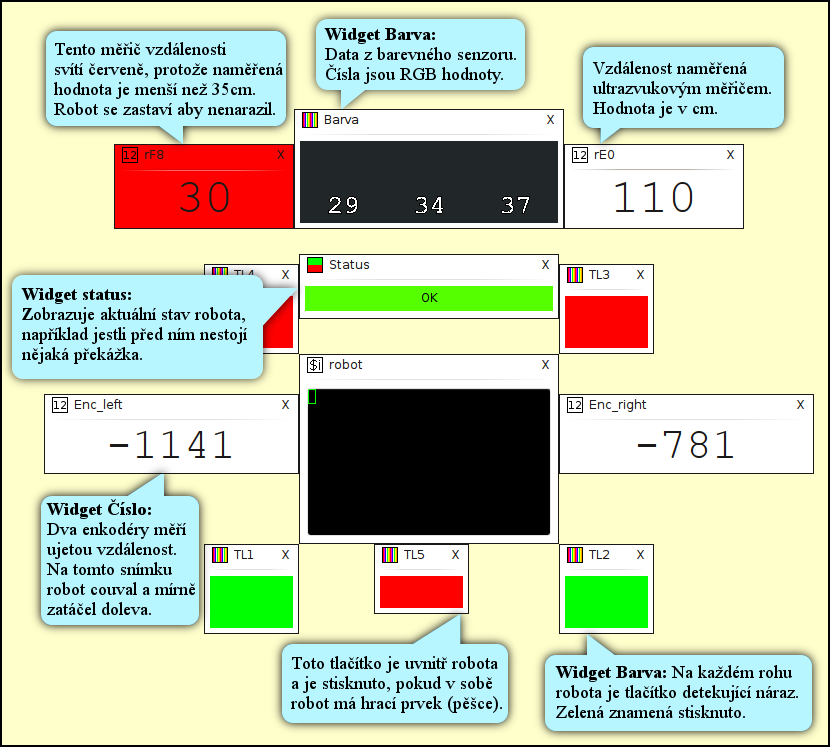
\includegraphics[width=\textwidth]{img/sensors_david.png}
\end{center}

\newpage
\subsubsection{Programování reaktivního chování robota}
Vrcholem vývoje robota bylo programování jeho chování na herní ploše. Při této příležitosti se v plné míře uplatnil widget \It{Script} programu Lorris. V tomto widgetu bylo vytvořeno scriptovací prostředí, které zapouzdřilo nejtypičtější povelové sady, pomocí kterých lze s výhodou konstruovat složitější vzorce chování robota. Widget \It{Script} by umožnil i přímé psaní scriptu pro řízení robota, ale zmíněné prostředí tuto práci výrazně zjednodušilo.

Za povšimnutí stojí také to, že zde byl widget script využit nejen pro řízení robota, ale i pro vylepšení fungování samotného nástroje Analyzér.

V tomto příkladu používám jednoduché \uv{akce}, které robot postupně provádí. Každá akce má 3 hlavní parametry - směr jízdy, kdy se má robot zastavit a co má vykonat, když se zastaví na cílovém místě. Všechny akce je možné ve scriptovacím prostředí rovnou měnit, bez nutnosti přeprogramovávat robota. Všechny ostatní části prostředí Lorris stále fungují, i když robot je právě řízen nastaveným scriptem. Díky tomu lze sledovat stav robota i všech jeho senzorů a rychle zjistit zdroj případného neočekávaného chování.
\\
\\
\noindent\It{Obrázek č. \ref{david_ctrl}, který patří této části textu, najdete v přílohách na straně \pageref{david_ctrl}.}

\newpage
\section{Aplikace pro Android}
\begin{figure}[H]
\begin{center}
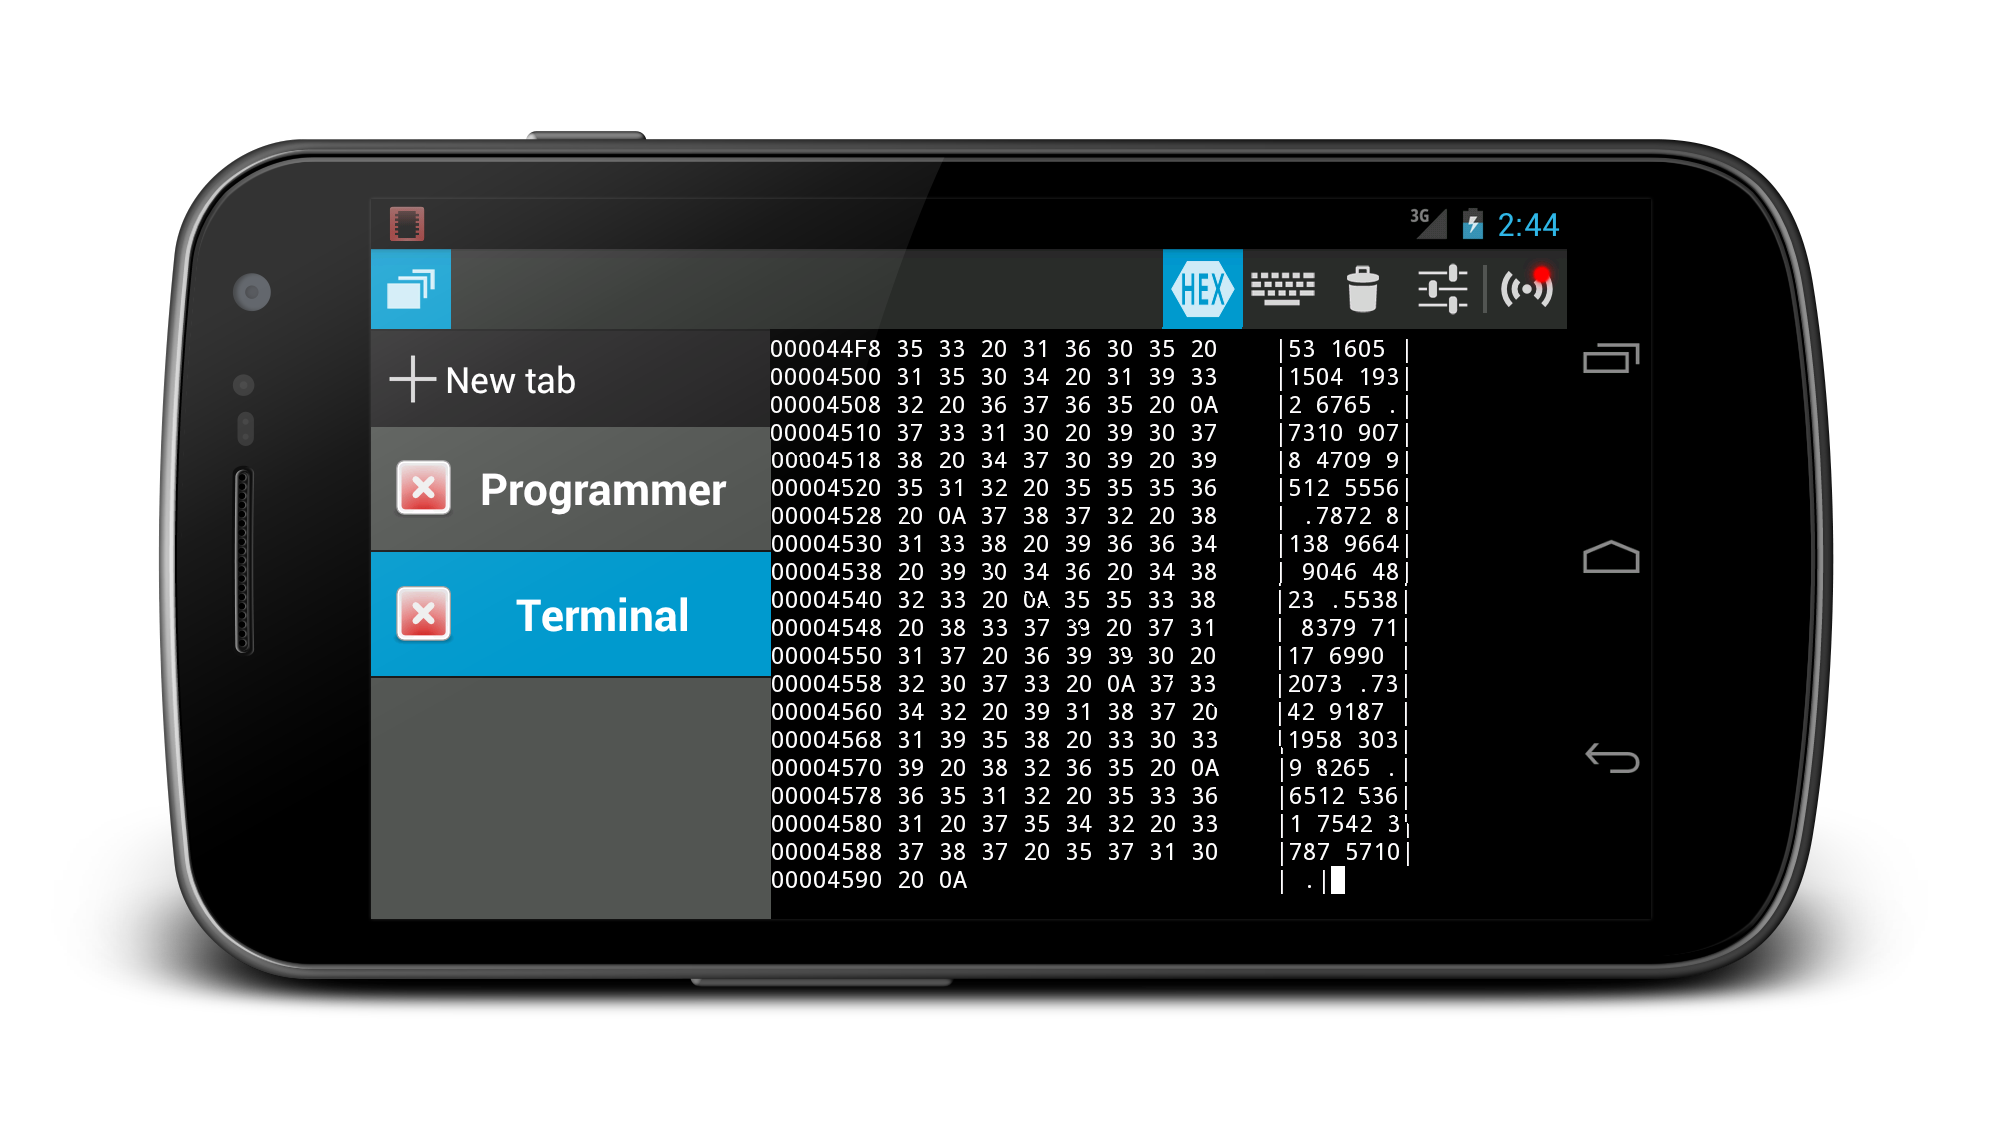
\includegraphics[width=\textwidth]{img/mobile.png}
\caption{Lorris mobile}
\end{center}
\end{figure}
Jako další vývojový stupeň jsem začal s vývojem Lorris pro platformu Google Android\cite{android}, protože chytrá zařízení s tímto operačním systémem jsou často při ruce a stačí k rychlému vyřešení menšího problému.

Aplikace {\bf Lorris mobile} slouží jako přenosný doplněk k počítačové verzi Lorris -- nemusí nutně obsahovat všechny funkce desktopové aplikace ale má pomoci zejména když je v terénu potřeba rychle něco přenastavit či poupravit.

Aplikace funguje na telefonech a tabletech s OS Android ve verzi 2.2 a vyšší, je optimalizována i pro větší obrazovky tabletů a je dostupná v oficiálním distribučním kanále Android aplikací -- v obchodě Google Play\cite{gplay}, stačí hledat heslo \uv{Lorris}.

Lorris mobile má podobnou architekturu jako desktopová verze Lorris. Začíná se vytvořením sezení, do kterého se ukládá vše, co uživatel v aplikaci otevře (obrázek \ref{mobile_session}). Po vytvoření a otevření sezení se uživatel dostane na hlavní obrazovku programu, kde si může otevřít jednotlivé moduly v záložkách podobně jako v desktopové aplikaci (obrázek \ref{mobile_tabs}).

\begin{figure}[H]
\begin{center}
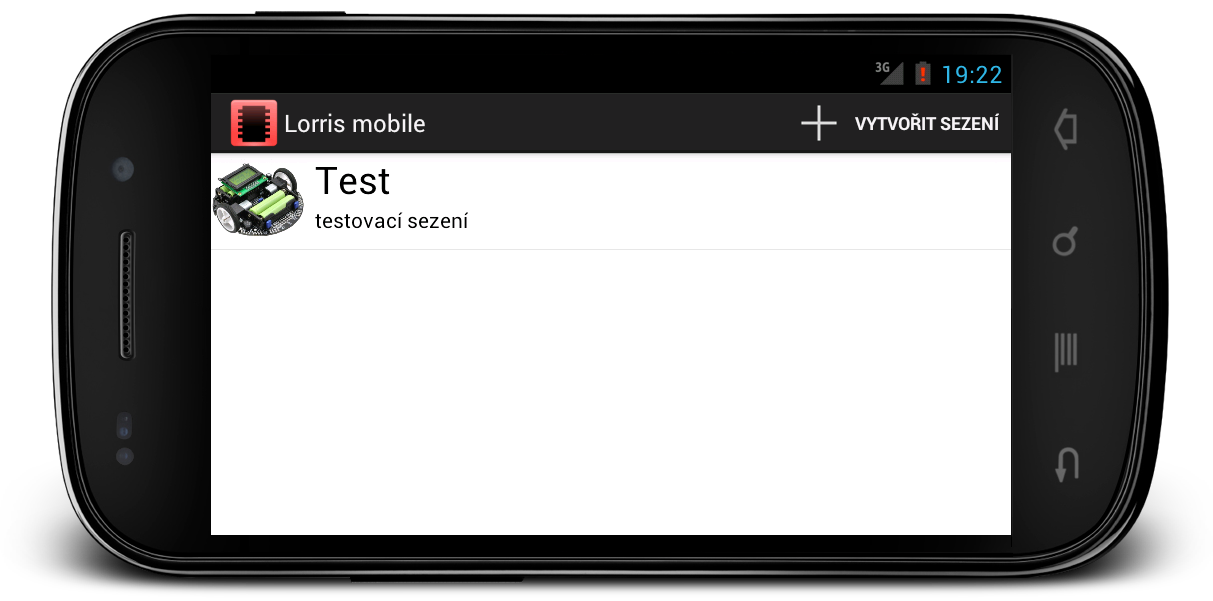
\includegraphics[width=\textwidth]{img/mobile_session.png}
\caption{Lorris mobile - výběr sezení}
\label{mobile_session}
\end{center}
\end{figure}
\begin{figure}[H]
\begin{center}
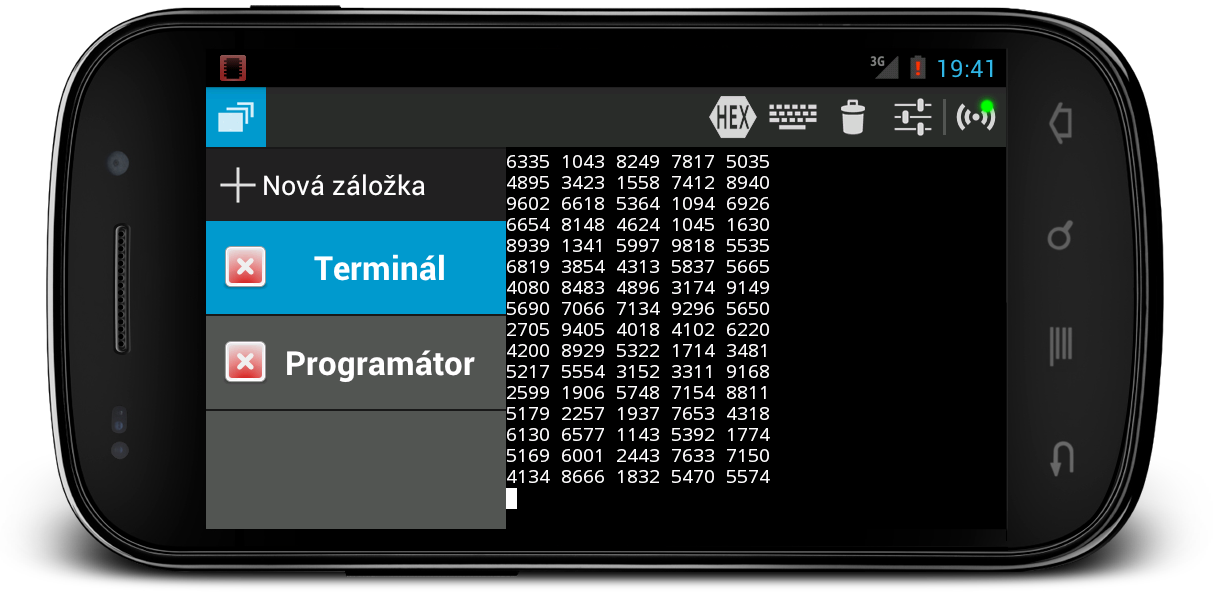
\includegraphics[width=\textwidth]{img/mobile_tabs.png}
\caption{Lorris mobile - přepínání záložek}
\label{mobile_tabs}
\end{center}
\end{figure}

\subsection{Programátor}
\begin{figure}[H]
\begin{center}
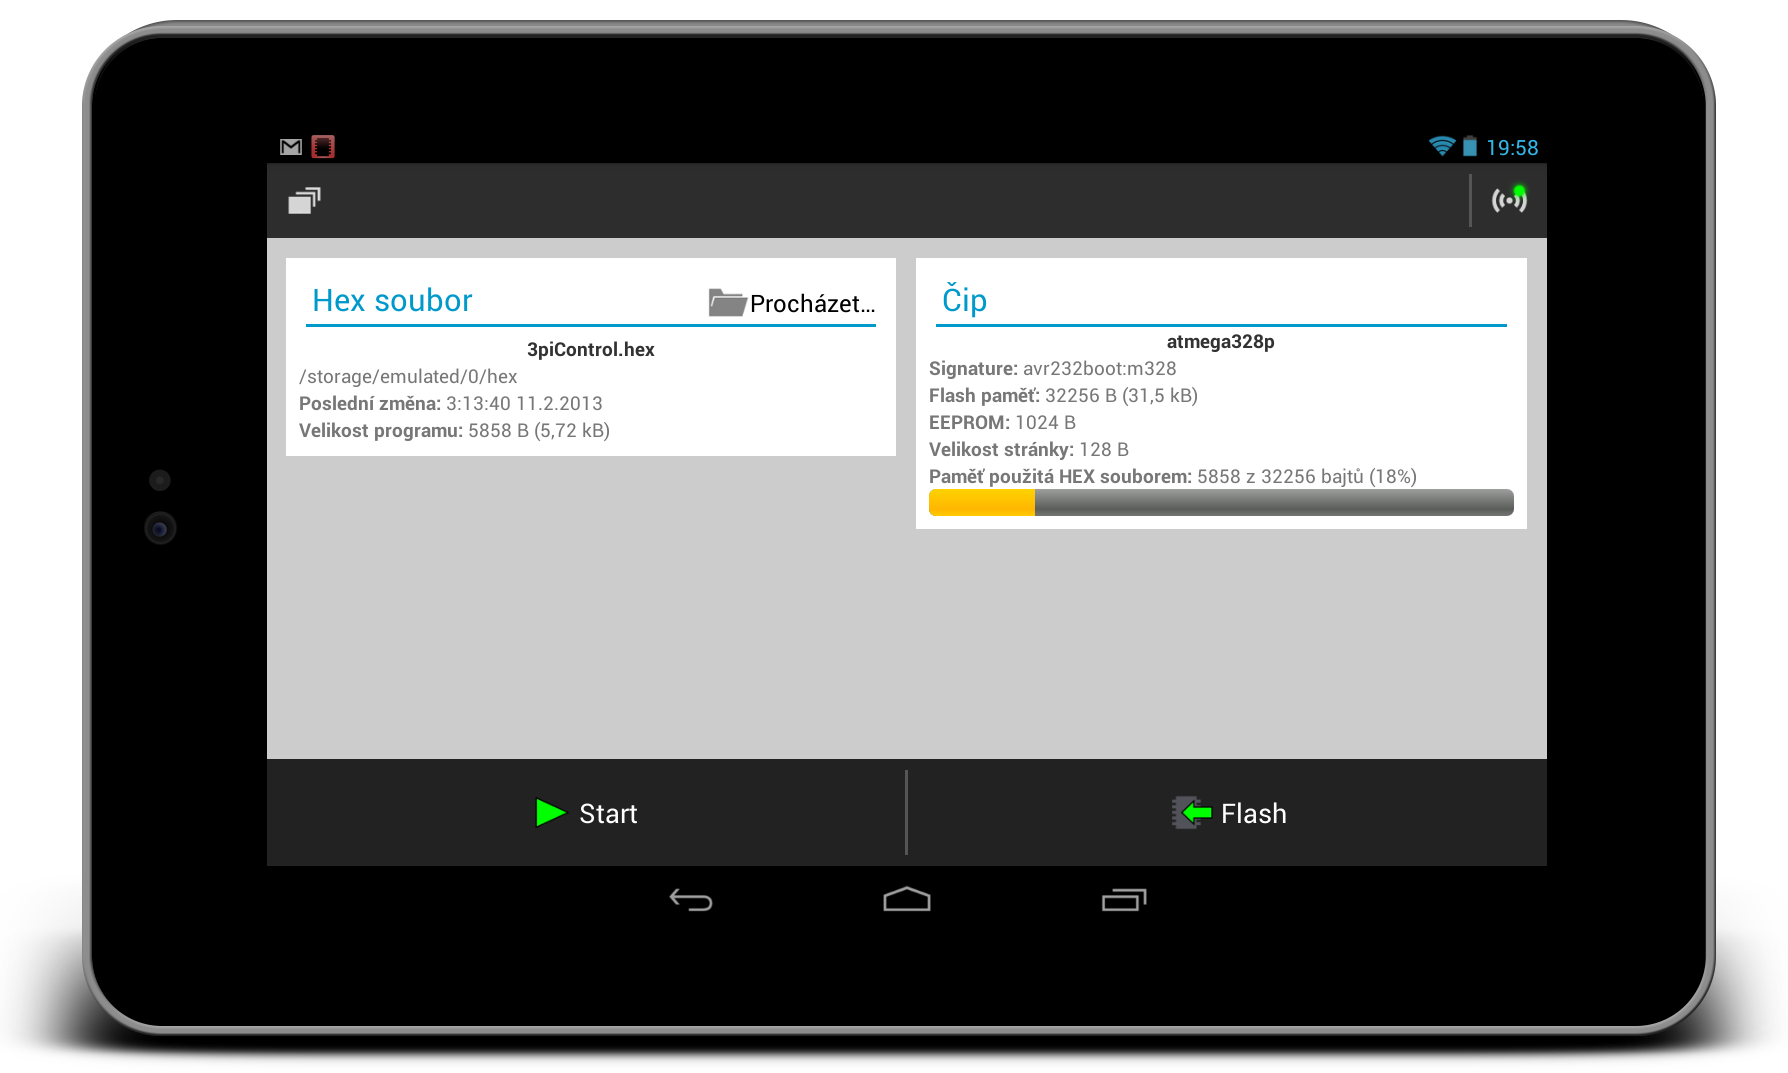
\includegraphics[width=\textwidth]{img/mobile_programmer.png}
\caption{Lorris mobile - programátor}
\end{center}
\end{figure}
Modul programátor dokáže programovat čipy pomocí bootloaderů {\bf avr232boot} a {\bf AVROSP} a také pomocí programátoru Shupito.
Tato část Lorris mobile používá části nativního kódu z desktopové verze Lorris, díky tomu se kód lépe spravuje a je rychlejší.

\subsection{Terminál}
\begin{figure}[H]
\begin{center}
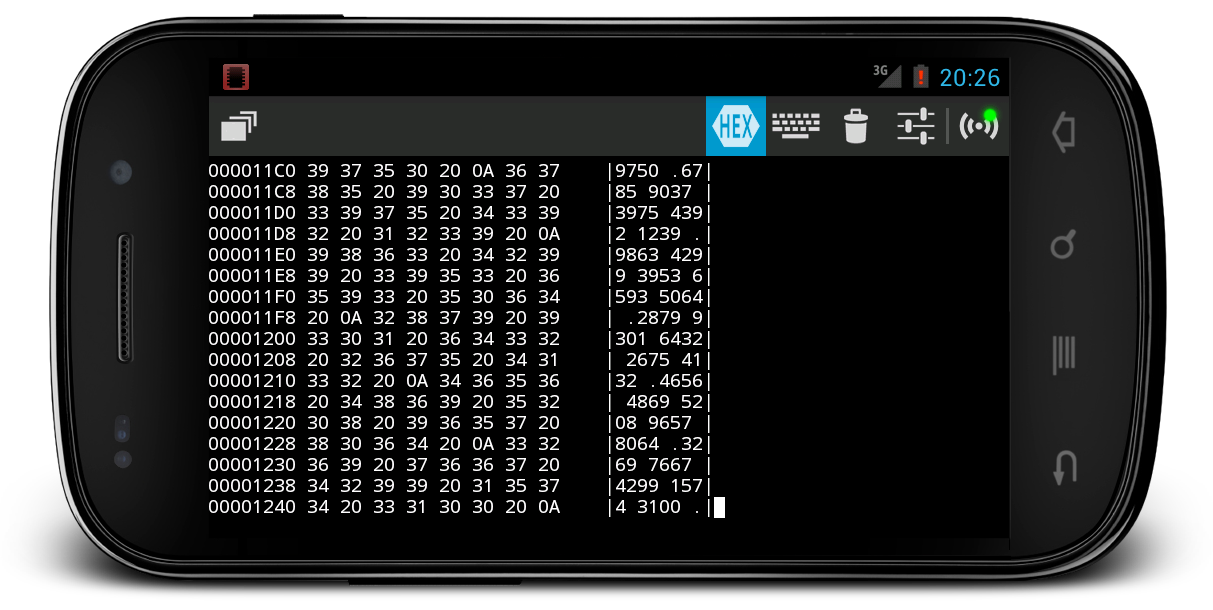
\includegraphics[width=\textwidth]{img/mobile_term.png}
\caption{Lorris mobile - terminál}
\end{center}
\end{figure}
Tento modul představuje běžný textový terminál. Umí většinu funkcí terminálu v desktopové verzi Lorris -- zobrazuje data (jako text nebo hexadecimální hodnoty bajtů), odesílá stisky kláves, lze nastavit velikost a barva textu, barvu pozadí a jaké kontrolní znaky se mají odeslat při stisknutí klávesy enter. 

\newpage
\section*{Závěr}
\addcontentsline{toc}{section}{Závěr}
Po několikaletém vývoji mohu konstatovat že aplikace splňuje všechny požadavky požadavky stanovené v kapitole \ref{motivace}:
\begin{enumerate}[label=\Has\hspace{1.5mm}\arabic{*}.] 
    \item Možnost zpracovávat data přicházející ze zařízení a přehledně je zobrazovat% 1
    \item Podpora co nejvíce formátů příchozích dat% 2
    \item Snadné a rychlé používání % 3
    \item Možnost běhu i na jiných systémech než je MS Windows % 4
    \item Co možná nejnižší cena -- program je dostupný zdarma% 5
    \item Snadná rozšířitelnost (ideálně otevřený zdrojový kód) % 6
    \item Nezávislost na další aplikaci (např. MS Office Excel) % 7
\end{enumerate}
Program navíc výrazně přesáhl původní cíle -- kromě zobrazování dat dokáže posílat data i zpět do zařízení, programovat mikročipy a vytvořit proxy mezi sériovým portem a TCP socketem. Ve srovnání s~nalezenými programy s~podobným zaměřením (viz úvod) je také jediný, který umožňuje uživateli napsat vlastní script pro parsování dat.

Lorris již má za sebou řadu ostrých nasazení a také rozšiřující se okruh věrných uživatelů, jak je podrobněji popsáno v kapitole \ref{usage}.

Aplikace je nadále vyvíjena, mohu prakticky donekonečna přídávat buďto další typy widgetů do modulu Analyzér (například kompas, směrový kříž, ...) nebo celé nové moduly (například rozhraní pro novou levnou logickou sondu, kterou vyvíjí Martin Vejnár). Program má v současné době (4.3.2013) asi 32 tisíc řádků kódu (bez knihoven třetích stran).

Přiložené CD obsahuje zdrojový kód, instruktážní video, propagační poster a anglickou verzi textu.
\begin{figure}[H]
\begin{center}
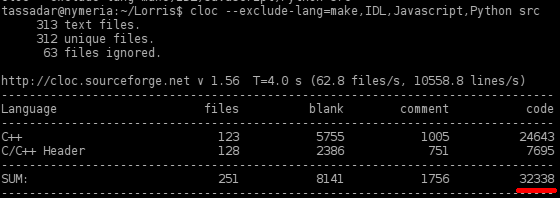
\includegraphics[width=\textwidth]{img/cloc_edit.png}
\caption{Počet řádků spočítaný programem CLOC\cite{cloc}}
\end{center}
\end{figure}


V budoucnu bych rád pokračoval v přidávání dalších funkcí do počítačové i mobilní verze Lorris a případně také v rozšiřování povědomí o celém balíku.


\subsection*{Reálné nasazení}
\label{usage}
%Já používám Lorris kdykoliv potřebuji naprogramovat, přenastavit či jinak
Prvními uživateli sady Lorris se stali od samého začátku vývoje před několika lety členové některých technicky zaměřených kroužků na DDM Junior\cite{junior} v Brně. Lorris zde pomáhá při stavbě různých zařízení, zejména robotů, a žáci, kteří se učí programovat mikrokontroléry, používají programátor \It{Shupito} a tím pádem i modul Programátor z balíku Lorris. V průběhu výuky programování mikrokontrolérů pomáhá také modul Terminál (jednoduchá komunikace s čipem) a později i Analyzér (pokročilé zpracovávání dat z čipu).

Lorris je pro použití v DDM Junior vhodná také díky nulové pořizovací ceně -- větší firma, zabývající se vývojem aplikací pro mikrokontroléry, by pravděpodobně pořídila drahý komerční program s podobnými funkcemi jako má Lorris nebo vyvinula vlastní jednoúčelové aplikace. Pro příspěvkové organizace typu DDM je však řešení používané velkými firmami poněkud nedostupné.

K dnešnímu dni má Lorris přibližně 20 uživatelů jen z řad DDM Junior. Díky postupnému rozšiřování programátoru \It{Shupito} mezi uživatele po celé ČR se ale okruh uživatelů Lorris utěšeně rozrůstá.

\vspace{10mm}

\noindent Já Lorris používám kdykoliv pracuji s roboty a mikrokontroléry -- pro zobrazování dat, programování mikročipů či ovládání celých zařízení. Následující seznam představuje pouze několik významnějších aplikací, pro které již byla sada Lorris použita ostatními uživateli:
\begin{itemize}
    \item Vývoj několika robotů pro soutěže letošního Robotického dne\cite{rob_den_new}
    \item Programování velkého počtu typů mikročipů, ať už pomocí programátoru \It{Shupito} nebo pomocí bootloaderů
    \item Vývoj samotného programátoru \It{Shupito}
    \item Já používám desktopovou Lorris ke generování testovacích dat pro mobilní verzi Lorris
    \item Vývoj levné logické sondy
    \item Ladění čipů pro ovládání třífazového motoru (tzv. \It{driver})
    \item Vývoj systému pro řízení až 128 RGB diod pro osvětlení modelu letadla
    \item Stavba a programování digitální vysílačky používající ARM procesor (semestrální práce)
    \item Vývoj robota pro sledování čáry (maturitní práce)
\end{itemize}





%%%%%%%%%%%%%%%%%%%%%%%%%%%%%%%%%%%%%%%%%%%%%%%%%%%%%%%%%%%%%%%%%%%%%%%%%%%
\newpage

%\section*{PŘÍLOHY}
%\addcontentsline{toc}{section}{PŘÍLOHY}

\section*{PŘÍLOHA A:}
\section*{Reference k widgetu \It{script}}
\addcontentsline{toc}{section}{PŘÍLOHA A: Reference k widgetu \It{script}}
\label{script_ref}
Widget \It{script} umožňuje parsování dat pomocí scriptu, který se píše v QtScriptu, který je založený na standardu ECMAScript, na kterém je založený JavaScript. Jazyk je hodně podobný JavaScriptu a většinou můžete použít jeho referenci. Tento text předpokládá alespoň základní znalost JavaScriptu nebo podobného programovacího jazyku.

\begin{itemize}
    \item \url{http://en.wikipedia.org/wiki/ECMAScript}
    \item \url{https://qt-project.org/doc/qt-4.8/scripting.html}
    \item \url{http://www.w3schools.com/jsref/default.asp} -- JS reference
\end{itemize}

\subsubsection*{Online dokumentace}
Ke scriptu je dostupná automaticky generovaná dokumentace, který obsahuje všechny dostupné metody a příklady scriptů:
\begin{itemize}
\item \url{http://technika.junior.cz/docs/Lorris}
\end{itemize}

\newpage
\subsection*{Základní script}
\addcontentsline{toc}{subsection}{Základní script}
Script by může obsahovat následující funkce (ale nemusí, pokud je nepoužívá):
\begin{listing}[H]
\begin{jscode}
function onDataChanged(data, dev, cmd, index) {
    return "";
}

function onKeyPress(key) {
}

function onRawData(data) {
}

function onWidgetAdd(widget, name) {
}

function onWidgetRemove(widget, name) {
}

function onScriptExit() {
}

function onSave() {
}
\end{jscode}
\caption{Základní script}
\label{input_script}
\end{listing}

\noindent{\color{blue}\verb/onDataChanged(data, dev, cmd, index)/} je volána při změně pozice v datech (tj. když přijdou nová data nebo uživatel pohne posuvníkem historie). Může vracet \verb/string/, který se přidá do terminálu.

\begin{itemize}
    \item \verb/data/ -- {\bf pole s Integery} obsahující příchozí data
    \item \verb/dev/ -- {\bf Integer} s ID zařízení (může být definováno v hlavičce packetu -- pokud není, \verb/dev/ se rovná -1)
    \item \verb/cmd/ -- {\bf Integer} s ID příkazu (může být definováno v hlavičce packetu -- pokud není, \verb/cmd/ se rovná -1)
    \item \verb/index/ -- {\bf Integer} s indexem packetu v příchozích datech.
\end{itemize}

\noindent{\color{blue}\verb/onKeyPress(key)/} je volána po stisku klávesy v terminálu.
\begin{itemize}
    \item \verb/key/ -- {\bf String} se stisknutou klávesou
\end{itemize}

\noindent{\color{blue}\verb/onRawData(data)/} je volána kdykoliv příjdou nějáká data.
\begin{itemize}
    \item \verb/data/ -- {\bf pole s bajty} obsahují nenaparsovaná data
\end{itemize}

\noindent{\color{blue}\verb/onWidgetAdd(widget, name)/} \\
{\color{blue}\verb/onWidgetRemove(widget, name)/}

jsou volány při přidání/odebrání widgetu z plochy
\begin{itemize}
    \item \verb/widget/ -- {\bf objekt} widgetu
    \item \verb/name/ -- {\bf String} se jménem widgetu
\end{itemize}

\noindent{\color{blue}\verb/onScriptExit()/} -- tato funkce je volána při ukončení scriptu. Je určena pro ukládání nastavení scriptu.

\noindent{\color{blue}\verb/onSave()/} -- tato funkce je volána těsně prěd uložením dat analyzéru. Je určena pro ukládání nastavení scriptu.

\subsection*{Základní funkce}
\addcontentsline{toc}{subsection}{Základní funkce}
Jsou dostupné základní javascriptové knihovny (\verb/Math/, \verb/Date/, ...) a samotná Lorris poskytuje další rozšiřující funkce. 

\begin{itemize}
    \item {\color{blue}\verb/appendTerm(String)/} -- přidá do terminálu text.\\
        \begin{listing}[H]
        \begin{jscode}
function onKeyPress(key) {
    appendTerm(key); // vypise _key_ do terminalu
}
        \end{jscode}
        \caption{Vypsání stisknutých kláves do terminálu}
        \end{listing}

    \item {\color{blue}\verb/clearTerm()/} -- vyčistí terminál.\\
        \begin{listing}[H]
        \begin{jscode}
function onKeyPress(key) {
    if(key == "c")
        clearTerm(); // vycisti terminal
    else
        appendTerm(key); // vypise _key_ do terminalu
}
        \end{jscode}
        \caption{Vypsání stisknutých kláves do terminálu a jeho vyčištění po stisku klávesy C}
        \end{listing}

    \item {\color{blue}\verb/sendData(pole Integerů)/} \\
         {\color{blue}\verb/sendData(String)/} -- pošle data do zařizení\\
        \begin{listing}[H]
        \begin{jscode}
function onKeyPress(key) {
    sendData(key);
}
        \end{jscode}
        \caption{Poslání ASCII kódu stisknuté klávesy}
        \end{listing}

    \item {\color{blue}\verb/throwException(String)/} -- zobrazí vyskakovací okno s hláškou

    \item {\color{blue}\verb/moveWidget(widget, int x, int y)/} \\
    {\color{blue}\verb/resizeWidget(widget, int sirka, int vyska)/} \\
        Tyto funkce přesunou/změní velikost widgetu. \verb|X| a \verb|Y| jsou absolutní hodnoty na ploše widgetů.

    \item {\color{blue}\verb/newWidget()/} -- tato funkce potřebuje o něco obsáhlejší popis, který je v následující kapitole
\end{itemize}

\subsection*{Vytvoření widgetu}
\addcontentsline{toc}{subsection}{Vytvoření widgetu}

Script může vytvořit všechny ostatní typy widgetů a posílat do nich data. 
{\color{blue}
\begin{verbatim}newWidget(typ, "jméno");
newWidget(typ, "jméno", šířka, výška);
newWidget(typ, "jméno", šířka, výška, Xoffset, Yoffset);
\end{verbatim}
}

\begin{itemize}
    \item \verb|typ| -- {\bf konstanta}, typ widgetu. Používají se tyto konstanty:
    \begin{verbatim}
    WIDGET_NUMBER, WIDGET_BAR, WIDGET_COLOR, WIDGET_GRAPH,
    WIDGET_SCRIPT, WIDGET_INPUT, WIDGET_TERMINAL, WIDGET_BUTTON,
    WIDGET_CIRCLE, WIDGET_SLIDER, WIDGET_CANVAS, WIDGET_STATUS
    \end{verbatim}
    \item \verb/jméno/ -- {\bf String}, jméno widgetu, zobrazí se v titulku
    \item \verb/šířka/ -- {\bf Integer}, šířka widgetu v pixelech. Může být 0, poté se zvolí minimální velikost.
    \item \verb/výška/ -- {\bf Integer}, výška widgetu v pixelech. Může být 0, poté se zvolí minimální velikost.
    \item \verb/Xoffset/ -- {\bf Integer}, vodorovná vzdálenost v pixelech od levého horního rohu mateřského ScriptWidgetu. Pokud není tento paramter zadán, vytvoří se nový widget v levém horním rohu aktuálně viditelné plochy.
    \item \verb/Yoffset/ -- {\bf Integer}, svislá vzdálenost v pixelech od levého horního rohu mateřského ScriptWidgetu. Pokud není tento paramter zadán, vytvoří se nový widget v levém horním rohu aktuálně viditelné plochy.
\end{itemize}

\begin{listing}[H]
\begin{jscode}
var cislo = newWidget(WIDGET_NUMBER,
                "rychlost", 200, 100, -250, 0);

function onDataChanged(data, dev, cmd, index) {
    cislo.setValue(data[0]);
    return "";
}
\end{jscode}
\caption{Vytvoření widgetu \It{číslo} a nastavení jeho hodnoty z příchozích dat}
\end{listing}

\subsection*{Dostupné funkce widgetů}
\addcontentsline{toc}{subsection}{Dostupné funkce widgetů}
Objekt widgetu je podtřídou třídy z Qt Frameworku QWidget -- díky tomu může používat jeho vlastnosti a sloty. Popis vlastností najdete v Qt referenci\footnote{\url{http://qt-project.org/doc/qt-4.7/qwidget.html\#propertySection}} v kapitole \uv{Properties} a ve scriptu se používají takto:

\begin{listing}[H]
\begin{jscode}
var cislo = newWidget(WIDGET_NUMBER,
                "rychlost", 200, 100, -250, 0);
cislo.visible = false; // skryti widgetu
\end{jscode}
\caption{Vytvoření widgetu \It{číslo} a nastaveni vlastnosti \uv{visible}}
\end{listing}
Popis slotů je taktéž v Qt referenci, tentokrát pod kapitolou \uv{Public slots}. Používají se jako metody:

\begin{listing}[H]
\begin{jscode}
var cislo = newWidget(WIDGET_NUMBER,
                "rychlost", 200, 100, -250, 0);
cislo.setDisabled(true); // znemozneni interakce s widgetem
\end{jscode}
\caption{Vytvoření widgetu \It{číslo} a použití slotu}
\end{listing}

Kromě těchto zděděných vlastností a funkcí má každý typ widgetu své vlastní.

%\newpage
\subsubsection*{Widget číslo}
\addcontentsline{toc}{subsubsection}{Widget číslo}
\begin{itemize}
    \item {\color{blue}\verb/setValue(Integer nebo double)/} -- Nastaví hodnotu widgetu
    \item {\color{blue}\verb/setFormula(String)/} -- nastaví výraz pro přepočítávání hodnoty
    \item {\color{blue}\verb/setDataType(konstanta)/} -- Nastaví typ vstupu. Konstanty:
        \begin{verbatim}
NUM_UINT8, NUM_UINT16, NUM_UINT32, NUM_UINT64, 
NUM_INT8, NUM_INT16, NUM_INT32, NUM_INT64, 
NUM_FLOAT, NUM_DOUBLE
        \end{verbatim}
\end{itemize}

\begin{listing}[H]
\begin{jscode}
var cislo = newWidget(WIDGET_NUMBER,
                "test cislo", 200, 100, -250, 0);
cislo.setValue(40);
cislo.setFormula("%n-100");
...
cislo.setValue(3.14);
\end{jscode}
\caption{Nastavení hodnoty widgetu \It{číslo}}
\end{listing}

\subsubsection*{Widget sloupcový bar}
\addcontentsline{toc}{subsubsection}{Widget sloupcový bar}
\begin{itemize}
    \item {\color{blue}\verb/setValue(Integer)/} -- Nastaví hodnotu widgetu
    \item {\color{blue}\verb/setRange(Integer min, Integer max)/} -- Nastaví minimální a maximální hodnotu widgetu
    \item {\color{blue}\verb/setRotation(Integer)/} -- Nastaví rotaci sloupce. 0 pro svislou, 1 pro vodorovnou
    \item {\color{blue}\verb/setFormula(String)/} -- nastaví výraz pro přepočítávání hodnoty
    \item {\color{blue}\verb/getMin(), getMax(), getValue()/} -- vrací minimální, maximální a aktualní hodnotu
\end{itemize}

\begin{listing}[H]
\begin{jscode}
var bar = newWidget(WIDGET_BAR, "test bar");
bar.setRange(0, 100); // rozmezi hodnot 0 az 100
bar.setValue(45); // nastaveni hodnoty na 45
bar.setRotation(1); // otoceni na vodorovno
\end{jscode}
\caption{Nastavení hodnot widgetu \It{sloupcový bar}}
\end{listing}

\subsubsection*{Widget barva}
\addcontentsline{toc}{subsubsection}{Widget barva}
\begin{itemize}
    \item {\color{blue}\verb/setValue(Integer r, Integer g, Integer b)/} \\
    {\color{blue}\verb/setValue(String barva)/} \\
    {\color{blue}\verb/setValue(Integer rgb)/} \\
    {\color{blue}\verb/setValueAr(pole integerů)/} \\
        -- Nastaví barvu ve widgetu.
    \item {\color{blue}\verb/setColorType(konstanta)/} -- Nastavý formát vstupu. Konstanty:
        \begin{verbatim}
COLOR_RGB_8, COLOR_RGB_10, COLOR_RGB_10_UINT,
COLOR_GRAY_8, COLOR_GRAY_10
        \end{verbatim}
\end{itemize}

\begin{listing}[H]
\begin{jscode}
var clr = newWidget(WIDGET_COLOR, "test barva");
clr.setValue(255, 255, 0);
clr.setColorType(COLOR_RGB_10);
clr.setValue(543, 1023, 200);
\end{jscode}
\caption{Nastavení hodnot widgetu \It{barva}}
\end{listing}

\subsubsection*{Widget graf}
\addcontentsline{toc}{subsubsection}{Widget graf}
Tento widget se od ostatních poměrně výrazně liší -- je třeba nejdříve vytvořit křivku až té nastavovat hodnoty. Funkce samotného widgetu graf jsou tyto:
\begin{itemize}
    \item {\color{blue}\verb/addCurve(String jméno, String barva)/} -- Vytvoří a vrátí novou křivku. \verb/barva/ může být buďto html název (např. red, blue) nebo HTML hex zápis (např. \#FF0000)
    \item {\color{blue}\verb/removeCurve(String jméno)/} \\
        {\color{blue}\verb/removeAllCurves()/} \\
        Odebrání jedné nebo všech křivek
    \item {\color{blue}\verb/setAxisScale(bool proX, double min, double max)/} -- Nastaví měřítko os. \verb/proX/ je {\bf true} pokud nastavujete měřítko osy $x$
    \item {\color{blue}\verb/updateVisibleArea()/} -- Přesune pohled na nejvyšší hodnotu osy $x$
\end{itemize}

\noindent{\color{blue}\verb/addCurve(String jméno, String barva)/} vrátí křivku, která má tyto funkce:

\begin{itemize}
    \item {\color{blue}\verb/addPoint(Integer index, double hodnota)/} -- Vloží bod křivky. \verb/index/ určuje pořadí bodů (bod s indexem 0 bude vždy před bodem s indexem 50, i když bude vložen až po něm). Pokud bod se stejným indexem už existuje, je jeho hodnota změněna
    \item {\color{blue}\verb/clear()/} -- Smaže všechny body křivky
\end{itemize}

\begin{listing}[H]
\begin{jscode}
var graf = newWidget(WIDGET_GRAPH, "graf", 400, 250, -420, 0);
graf.setAxisScale(false, -105, 105); // meritko osy y
graf.setAxisScale(true, 0, 200); // meritko osy x

// vytvoreni krivky sin
var sin = graf.addCurve("sin", "blue"); 

// pridani bodu do krivky sin
var sinVal = 0;
for(var i = 0; i < 500; ++i) {
    sin.addPoint(i, Math.sin(sinVal)*100);
    sinVal += 0.1;
}
// presunuti na posledni hodnotu krivky
graf.updateVisibleArea(); 
\end{jscode}
\caption{Zobrazení křivky funkce sinus ve widgetu \It{graf}}
\end{listing}

\subsubsection*{Widget vstup}
\addcontentsline{toc}{subsubsection}{Widget vstup}
Tento widget lze vytvořit pouze ze scriptu a umí zobrazit a ovládat většinu Qt widgetů\footnote{\url{http://qt-project.org/doc/qt-4.7/widgets-and-layouts.html}}, například tlačítko (\verb/QPushButton/), zaškrtávací políčko (\verb/QCheckBox/) či textové políčko (\verb/QLineEdit/). Dokumentace k těmto widgetům je v Qt referenci, opět můžete používat vlastnosti (\uv{Properties}) a funkce (\uv{Public slots}).\\
Funkce widgetu \It{vstup}:
\begin{itemize}
    \item {\color{blue}\verb/newWidget(String jméno, Integer roztahování = 0)/} -- Vytvoří a vrátí nový QWidget. \verb/jméno/ musí být jméno třídy widgetu, například QPushButton, QCheckBox nebo QLineEdit. \verb/roztahování/ značí jak moc se bude widget roztahovat oproti ostatním.
    \item {\color{blue}\verb/removeWidget(Objekt widget)/} -- Odstraní widget vrácený voláním \verb|newWidget|.
    \item {\color{blue}\verb/clear()/} -- Odstraní všechny widgety.
    \item {\color{blue}\verb/setHorizontal(bool horizontal)/} -- Nastaví způsob uspořádání widgetů (vedle sebe nebo pod sebou).
\end{itemize}

\begin{listing}[H]
\begin{jscode}
var vstup = newWidget(WIDGET_INPUT,
                "test vstupu", 150, 100, -160, 0);
var label = vstup.newWidget("QLabel", 1);

// zarovnani textu na stred. 
// 0x0080 a 0x0004 jsou konstanty Qt Frameworku 
// Qt::AlignHCenter a Qt::AlignVCenter
label.alignment = 0x0080 | 0x0004;

// nastaveni textu
label.text = "Testovaci popisek";
\end{jscode}
\caption{Widget \It{vstup} -- vytvoření QLabel}
\end{listing}
Widget vytvořený tímto příkladem vypadá takto:

\begin{figure}[H]
\begin{center}
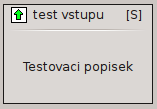
\includegraphics{img/ref_input.png}
\caption{Widget \It{vstup} -- vytvoření QLabel}
\end{center}
\end{figure}

\newpage
QtScript podporuje i využití principu signálů a slotů, díky tomu lze ve scriptu reagovat například na stisknutí tlačítka.

\begin{listing}[H]
\begin{jscode}
var vstup = newWidget(WIDGET_INPUT,
                "test vstupu", 150, 100, -160, 0);

var rychlost = vstup.newWidget("QLineEdit");
rychlost.text = "100";

var btn = vstup.newWidget("QPushButton", 1);
btn.text = "Nastavit";

function posliRychlost() {
    var speed = parseInt(rychlost.text);
    sendData(new Array(speed));
    appendTerm("Rychlost " + speed + "odeslana\n");
}
// Pripojeni signalu "clicked" na slot posliRychlost()
btn.clicked.connect(posliRychlost);
\end{jscode}
\caption{Widget \It{vstup} -- tlačítko}
\end{listing}

\begin{figure}[H]
\begin{center}
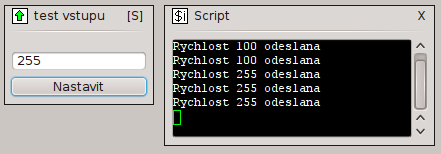
\includegraphics{img/ref_input2.png}
\caption{Widget \It{vstup} -- tlačítko}
\end{center}
\end{figure}

\subsubsection*{Widget kolo}
\addcontentsline{toc}{subsubsection}{Widget kolo}
\begin{itemize}
    \item {\color{blue}\verb/setValue(číslo)/} -- Nastaví zobrazený úhel
    \item {\color{blue}\verb/setClockwise(bool clockwise)/} -- Nastaví jestli se úhel počítá po nebo proti směru hodinových ručiček
    \item {\color{blue}\verb/setAngType(konstanta, min, max/} -- Nastavý vstupní formát. Konstanty:
\verb|ANG_RAD, ANG_DEG, ANG_RANGE|
\end{itemize}

\begin{listing}[H]
\begin{jscode}
var c = newWidget(WIDGET_CIRCLE, "kolo", 200, 200, -210, 0);

c.setAngType(ANG_DEG); // nastaveni vstupu na stupne
c.setValue(270);
\end{jscode}
\caption{Nastavení hodnot widgetu \It{kolo}}
\end{listing}

\subsubsection*{Widget plátno}
\addcontentsline{toc}{subsubsection}{Widget plátno}
\begin{itemize}
    \item {\color{blue}\verb/clear()/} -- Vymaže vše, co je ve widgetu namalované
    \item {\color{blue}\verb/setBackground(String barva)/} -- Nastaví barvu pozadí
    \item {\color{blue}\verb/drawLine(int x1, int y1, int x2, int y2)/} -- Nakreslí čáru.
    \item {\color{blue}\verb/drawLine(int x, int y)/} -- Nakreslí čáru. Začátek je v bodě, kde končí předchozí nakreslená čára (nebo v [0,0] pokud ještě nebyla žádná nakreslená).
    \item {\color{blue}\verb/drawRect(int x, int y, int sirka, int vyska)/} -- Nakreslí obdélník.
    \item {\color{blue}\verb/drawEllipse(int x, int y, int sirka, int vyska)/} -- Nakreslí elipsu
    \item {\color{blue}\verb/drawEllipse(int x, int y, int polomer)/} -- Nakreslí kruh
    \item {\color{blue}\verb/setLineSize(int tloušťka)/} -- Tloušťka čáry, kterou se prvky kreslí.
    \item {\color{blue}\verb/setLineColor(String barva)/} -- Barva čáry, kterou se prvky kreslí.
    \item {\color{blue}\verb/setFillColor(String barva)/} -- Barva výplně obdélníků, elips a kruhů
\end{itemize}

\begin{listing}[H]
\begin{jscode}
var c = newWidget(WIDGET_CANVAS, "Canvas", 140, 170, -150, 0);
c.setLineColor("red");
c.setFillColor("red");

c.drawRect(55, 10, 20, 110);
c.drawRect(10, 55, 110, 20);
\end{jscode}
\caption{Nakreslení kříže ve widgetu \It{plátno}}
\end{listing}

\begin{figure}[H]
\begin{center}
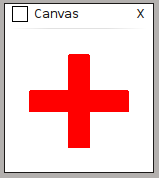
\includegraphics[scale=1]{img/w_canvas.png}
\caption{Nakreslení kříže ve widgetu \It{plátno}}
\end{center}
\end{figure}

\subsubsection*{Widget status}
\addcontentsline{toc}{subsubsection}{Widget status}
\begin{itemize}
    \item {\color{blue}
    \begin{verbatim}addStatus(int id, bool bitMaska, String text
    String barvaPozadí, String barvaTextu)
    \end{verbatim}} Přidá nový status. \verb|bitMask| určuje, zda se má použít přímé porovnání s hodnotou \verb|id| nebo bitový operátor \verb|AND|.
    \item {\color{blue}\verb/removeStatus(int id, bool bitMaska/} -- Odebere status
    \item {\color{blue}\verb/setValue(Integer)/} -- Nastaví vstupní hodnotu
    \item {\color{blue}\verb/getValue()/} -- Vrátí aktuální hodnotu
    \item {\color{blue}\verb/showStatusManager()/} -- Vyvolá dialog pro správu stavů ve widgetu
\end{itemize}

\begin{listing}[H]
\begin{jscode}
var s = newWidget(WIDGET_STATUS, "stav", 0, 0, 200, 0);

s.addStatus(2, false, "Porucha", "orange", "black");
s.setValue(2);
\end{jscode}
\caption{Ovládání widgetu \It{status} ze scriptu}
\end{listing}

\begin{figure}[H]
\begin{center}
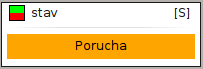
\includegraphics[scale=1]{img/status_script.png}
\caption{Ovládání widgetu \It{status} ze scriptu}
\end{center}
\end{figure}

\subsubsection*{Widget tlačítko}
\addcontentsline{toc}{subsubsection}{Widget tlačítko}
Kromě funkcí, které tento widget má je také možné nastavit metodu která se provede po kliknutí, stačí ve scriptu vytvořit metodu {\color{blue}\verb/JménoWidgetu_clicked()/}.
\begin{itemize}
    \item {\color{blue}\verb/setButtonName(String text)/} -- Nastaví text na tlačítku
    \item {\color{blue}\verb/setShortcut(String zkratka)/} -- Nastaví klávesovou zkratku pro tlačítko
    \item {\color{blue}\verb/setColor(String barva)/} -- Nastaví barvu tlačítka
    \item {\color{blue}\verb/setTextColor(String barva)/} -- Nastaví barvu textu na tlačítku
\end{itemize}

\begin{listing}[H]
\begin{jscode}
var t = newWidget(WIDGET_BUTTON, "tlacitko", 0, 0, 200, 0);

t.setButtonName("Pokus");
t.setShortcut("Ctrl+H");
t.setColor("white");

function tlacitko_clicked() {
    appendTerm("Tlacitko stisknuto!\n");
}
\end{jscode}
\caption{Nastavení widgetu \It{tlačítko} ze scriptu}
\end{listing}

\newpage
\subsubsection*{Widget slider}
\addcontentsline{toc}{subsubsection}{Widget slider}
Kromě funkcí, které tento widget má je také možné nastavit metodu která se provedou při různých změnách stavu slideru. Mají tvar  {\color{blue}\verb/JménoWidgetu_jmenoZmeny()/}, v následujícím příkladě má widget jméno \Uv{Slider}.
\begin{listing}[H]
\begin{jscode}
function Slider_valueChanged() {
    appendTerm("hodnota: " + Slider.getValue() + "\n");
}

function Slider_minimumChanged() {
    appendTerm("nove minimum: " + Slider.getMin() + "\n");
}

function Slider_maximumChanged() {
    appendTerm("nove maximum: " + Slider.getMax() + "\n");
}

function Slider_typeChanged() {
    appendTerm("Typ vstupu zmene na " +
        (Slider.isInteger() ? "Integer" : "Double") + "\n");
}

function Slider_orientationChanged() {
    appendTerm("orientace zmenena na " +
        Slider.getOrientation() + "\n");
}
\end{jscode}
\caption{Funkce, ktere jsou volány při změně stavu widgetu \It{slider}}
\end{listing}
\begin{itemize}
    \item {\color{blue}\verb/setType(bool double)/} -- Nastaví typ hodnot které widget nastavuje (celá nebo desetinná čísla).
    \item {\color{blue}\verb/setMin, setMax, setValue (číslo)/} -- Nastaví minimální, maximální a aktuální hodnotu
    \item {\color{blue}\verb/getMin(), getMax(), getValue()/} -- Vrátí minimální, maximální a aktální hodnotu
\end{itemize}

\begin{listing}[H]
\begin{jscode}
var s = newWidget(WIDGET_SLIDER, "Slider", 0, 0, 300, 0);

s.setType(true); // desetinna cisla
s.setMax(6.28);
s.setValue(3.14);

function Slider_valueChanged() {
    appendTerm("value changed: " + Slider.getValue() + "\n");
}
\end{jscode}
\caption{Ovládání wigetu \It{slider} ze scriptu}
\end{listing}

\newpage
\subsection*{Ukládání dat scriptu}
\addcontentsline{toc}{subsection}{Ukládání dat scriptu}
Na uložení hodnot použitých ve scriptu (například nastavení) je připravena třída \verb|ScriptStorage|. Ve scriptu je dostupná jako objekt \verb|storage| a má tyto funkce:
\begin{itemize}
    \item {\color{blue}\verb/clear()/} -- Vymaže všechna uložená dataPass
    \item {\color{blue}\verb/exists(String klíč)/} -- Vrátí \verb|true| pokud hodnota s tímto klíčem existuje.
    \item {\color{blue}\verb/setXXXX(String klíč, XXXX hodnota)/} \\
        {\color{blue}\verb/getXXXX(String klíč, XXXX pokudKlíčNeexistuje)/} \\
        {\color{blue}\verb/setYYYYArray(String klíč, PoleYYYY hodnota)/} \\
        {\color{blue}\verb/getYYYYArray(String klíč, PoleYYYY pokudKlíčNeexistuje)/} \\
            Funkce pro uložení a načtení hodnoty.

        \verb|XXX| typy mohou být \verb|Bool, UInt32, Int32, Float| nebo \verb|String|. Pole \verb|YYYY| může být s prvky typu \verb|UInt32, Int32| nebo \verb|Float|. Druhý parametr u \verb|getXXXX| metod je výchozí hodnota, která se vrátí pokud klíč neexistuje.
\end{itemize}

\begin{listing}[H]
\begin{jscode}
var s = newWidget(WIDGET_SLIDER, "Slider", 0, 0, 300, 0);
s.setType(true); // desetinna cisla
s.setMax(6.28);

// Nacte hodnotu, ktera byla pred tim ulozena v metode save()
var ulozene = storage.getFloat("hodnotaPosuvniku", 3.14);
s.setValue(ulozene);

// Nacte pokusne pole cisel ulozene v metode save()
var pokus = storage.getInt32Array("pokusnePole", new Array());
appendTerm("Ulozene pole: " + pokus + "\n");

function onSave() {
    save();
}

function onScriptExit() {
    save();
}

function save() {
    storage.setFloat("hodnotaPosuvniku", Slider.getValue());

    var pokus = new Array(4, 8, 15, 16, 23, 42);
    storage.setInt32Array("pokusnePole", pokus);
}
\end{jscode}
\caption{Ukládání dat scriptu}
\end{listing}

\newpage
\subsection*{Přístup k joysticku}
\addcontentsline{toc}{subsection}{Přístup k joysticku}
Nejříve několik globálních metod pro práci s joysticky:
\begin{itemize}
    \item {\color{blue}\verb/getJoystickNames()/} -- Vráti pole Stringů se jmény přípojených joysticků.
    \item {\color{blue}\verb/getJoystickIds()/} -- Vráti pole Integerů s ID připojených joysticků. Indexy v tomto poli korespondují s polem z funkce \verb|getJoystickNames()|, tj. ID na pozici 0 patří ke jménu na pozici 0.
    \item {\color{blue}\verb/getJoystick(int id)/} -- Otevře joystick s daným ID a vrací object \verb|Joystick| neno NULL pokud nebylo možné joystick otevřit.
    \item {\color{blue}\verb/closeJoystick(Joystick)/} -- Zavře a uvolní objekt joysticku
\end{itemize}
Objekt \verb|joystick| pak má následující metody:
\begin{itemize}
    \item {\color{blue}\verb/getId()/} -- Vrátí ID joysticku
    \item {\color{blue}\verb/getNumAxes()/} \\
          {\color{blue}\verb/getNumButtons()/} -- Vrátí počet os nebo tlačítek
    \item {\color{blue}\verb/getAxisVal(int osa)/} -- Vrátí aktuální hodnotu osy joysticku jako číslo mezi -32768 a 32767. Parametr \verb|osa| je číslo od 0 do \verb|getNumAxes()-1|.
    \item {\color{blue}\verb/getButtonVal(int tlačítko)/} -- Vrátí aktuální hodnotu tlačítka jako číslo 0 (uvolněno) nebo 1 (stisknuto). Parametr \verb|tlačítko| je číslo od 0 do \verb|getNumButtons()-1|.
\end{itemize}
Kromě toho má joystick také dva signály, na které se můžete ve scriptu napojit:
\begin{itemize}
    \item {\color{blue}\verb/axesChanged(Pole integerů)/} -- Volá se když se hodnota některé z os změní. V poli jsou indexy os které se změnily.
    \item {\color{blue}\verb/buttonChanged(int tlačítko, int stav)/} -- Volá se když se zmení stav tlačítka. Parametr \verb|tlačítko| je index tlačítka a \verb|stav| je číslo 0 nebo 1.
\end{itemize}

\begin{listing}[H]
\begin{jscode}
// Pokusi se otevrit prvni dostupny joystick
var ids = getJoystickIds();
var joy = getJoystick(ids[0]);

if(joy) {
    // pripojeni na signaly
    joy.axesChanged.connect(axesChanged);
    joy.buttonChanged.connect(buttonChanged);

    appendTerm("ID joysticku: " + joy.getId() + "\n");
    appendTerm("Pocet os: " + joy.getNumAxes() + "\n");
    appendTerm("Pocet tlacitek: " +
            joy.getNumButtons() + "\n");
}

function axesChanged(axes) {
    for(var i = 0; i < axes.length; ++i) {
        var hodnota = joy.getAxisVal(axes[i]);
        appendTerm("Osa " + axes[i] + ": " + hodnota + "\n");
    }
}

function buttonChanged(id, state) {
    appendTerm("Tlacitko " + id + ", stav: " + state + "\n");
}
\end{jscode}
\caption{Otevření joysticku a čtení jeho hodnot}
\end{listing}
%\newpage
%\subsection*{Pár věcí, na které je třeba při programování myslet}
%\addcontentsline{toc}{subsection}{Pár věcí na které je třeba myslet}
%\begin{itemize}
    %\item Widgety vytvořené ze scriptu se neukládají do datového souboru -- po načtení se vytvoří znovu, bez dat.
    %\item Stav proměnných ve scritptu se neukládá do souboru.
    %\item Po stisknutí \uv{Ok} nebo \uv{Použít} v dialogu nastavení scritpu se script načte znovu -- staré widgety vytvořené scriptem se smažou a vytvoří nové, bez dat.
    %\item Jazyk nemá žádné pojistky proti \uv{špatnému} kódu -- pokud ve scritpu bude nekonečná smyčka, Lorris prostě zamrzne
%\end{itemize}

\newpage
\section*{PŘÍLOHA B:}
\section*{Knihovny třetích stran}
\addcontentsline{toc}{section}{PŘÍLOHA B: Knihovny třetích stran}
\begin{itemize}
    \item {\bf Qwt}\cite{qwt} je knihovna pro Qt Framework obsahující tzv. widgety pro aplikace technického charakteru -- grafy, sloucové ukazatele, kompasy a podobně.
    \item {\bf QExtSerialPort}\cite{qext} poskytuje připojení k sériovému portu a také dokáže vypsat seznam nalezených portů v počítačí.
    \item {\bf QHexEdit2}\cite{qhex} je hex editor použitý v modulu programátor na zobrazování obsahu paměti. V této knihovně jsem upravoval několik málo drobností, týkajících se především vzhledu.
    \item {\bf Tanto Icon Library}\cite{tango} je sada ikon vydaných jako volné dílo. Lorris použivá ikonky z této sady na mnoha místech napříč celým programem.
    \item {\bf EcWin7}\cite{ecwin7} je knihovna, která poskytuje API k progressbaru v hlavním panelu Windows 7.
    \item {\bf QScintilla2}\cite{qsci} je pokročilý editor textu pro Qt.
    \item {\bf PythonQt}\cite{pythonqt} jsou Python bindings pro Qt.
    \item {\bf Python}\cite{python} je programovací jazyk, používají se některé části jeho interpreteru v kombinaci s PythonQt.
    \item {\bf Qt Solutions}\cite{qtsolutions} je soubor několika přídavných modulů pro Qt
    \item {\bf libyb}\cite{libyb} je knihovna která obstarává komunikaci s programátorem Shupito
\end{itemize}

\section*{PŘÍLOHA C:}
\section*{Licence}
\addcontentsline{toc}{section}{PŘÍLOHA C: Licence}
Lorris je dostupný pod licencí GNU GPLv3\cite{gpl3}, licence použitých programů a knihoven jsou následující:
\begin{itemize}
    \item {\bf Qt Framework} je distribuován pod licencí GNU LGPLv2.1\cite{lgpl}
    \item {\bf Qwt} je distribuováno pod Qwt license\cite{qwtlicense}, která je založená na GNU LGPLv2.1
    \item {\bf QExtSerialPort} je distribuován pod The New BSD License\cite{newbsd}
    \item {\bf QHexEdit2} je distribuován pod licencí GNU LGPLv2.1
    \item {\bf Tanto Icon Library}\cite{tango} je vydána jako volné dílo (\It{Public domain})
    \item {\bf EcWin7} je distribuováno pod GNU GPLv2
    \item {\bf QScintilla2} je distribuována pod GNU GPL v2 a v3
    \item {\bf libenjoy}\cite{libenjoy} je distribuována pod GNU LGPLv2.1
    \item {\bf PythonQt} je distribuována pod GNU LGPLv2.1
    \item {\bf Python} je distribuován pod PSF License agreement\cite{psf}
    \item {\bf Qt Solutions} je distribuován pod The New BSD License
    \item {\bf libyb} je distribuován pod Boost Software License\cite{boost}
\end{itemize}

Všechny tyto licence umožňují svobodné používání a šíření kódu.

\newpage
 \section*{PŘÍLOHA D:}
 \begin{thebibliography}{99}
\addcontentsline{toc}{section}{PŘÍLOHA D: Reference}
 %% 99 znamená, že maximální délka čísla literatury jsou dva znaky
% seznam samozřejmě změníte podle svého, tohle je pouze ukázka formátování

    \bibitem{serialchart} \It{SerialChart} -- Analyse and chart serial data from RS-232 COM ports \\
    \url{http://code.google.com/p/serialchart/}\\
    (Stav ke dni 25.2.2013)

    \bibitem{winwedge} \It{WinWedge} -- RS232 data collection software \\
    \url{http://www.taltech.com/products/winwedge/}\\
    (Stav ke dni 25.2.2013)

    \bibitem{serialdatalogger} \It{Advanced Serial Data Logger} \\
    \url{http://www.aggsoft.com/serial-data-logger.htm}\\
    (Stav ke dni 25.2.2013)

    \bibitem{stamplot} \It{StampPlot Pro} -- Graphical Data Acquisition and Control \\
    \url{http://www.selmaware.com/stampplot/index.htm}\\
    (Stav ke dni 25.2.2013)

    \bibitem{qtfrm} \It{Qt} -- Cross--platform application and UI framework \\
    \url{http://qt-project.org/}\\
    (Stav ke dni 25.2.2013)

    \bibitem{debian} \It{Debian Linux} -- The Universal Operating System \\
    \url{http://www.debian.org/}\\
    (Stav ke dni 25.2.2013)

    \bibitem{github} \It{GitHub} -- Social Coding \\
    \url{https://github.com}\\
    (Stav ke dni 25.2.2013)

    \bibitem{qtscript} \It{Making Applications Scriptable} \\
    \url{http://qt-project.org/doc/qt-4.8/scripting.html}\\
    (Stav ke dni 25.2.2013)

    \bibitem{sdl} \It{SDL} -- Simple Directmedia Layer \\
    \url{http://www.libsdl.org/}\\
    (Stav ke dni 13.2.2013)

    \bibitem{3pi} \It{Pololu 3pi Robot} \\
    \url{http://www.pololu.com/catalog/product/975}\\
    (Stav ke dni 25.2.2013)

    \bibitem{rob_den} \It{Robotický den 2012} \\
    \url{http://www.robotickyden.cz/2012/}\\
    (Stav ke dni 25.2.2013)

    \bibitem{robotday_res} \It{Robotický den 2012} -- výsledky soutěže Line Follower standard\\
    \url{http://www.robotickyden.cz/2012/results/lfs.php}\\
    (Stav ke dni 28.2.2013)

    \bibitem{eurobot} \It{Eurobot} \\
    \url{http://www.eurobot.org/}\\
    (Stav ke dni 25.2.2013)

    \bibitem{eurobot11} \It{Eurobot 2011} \\
    \url{http://www.eurobot.cz/eurobot2011.php}\\
    (Stav ke dni 25.2.2013)

    \bibitem{junior} \It{DDM Junior, Dornych 2, Brno, 656 20}\\
    \url{http://www.junior.cz}\\
    (Stav ke dni 4.3.2013)

    \bibitem{rob_den_new} \It{Robotický den} \\
    \url{http://www.robotickyden.cz/}\\
    (Stav ke dni 4.3.2013)

    \bibitem{android} \It{Google Android} -- Operační systém pro chytré telefony\\
    \url{http://www.android.com/}\\
    (Stav ke dni 25.2.2013)

    \bibitem{gplay} \It{Google Play Store} -- Obchod s aplikacemi pro OS Android\\
    \url{http://play.google.com/store}\\
    (Stav ke dni 14.2.2013)

    \bibitem{cloc} \It{CLOC} -- Count Lines of Code \\
    \url{http://cloc.sourceforge.net/}\\
    (Stav ke dni 25.2.2013)

    \bibitem{qwt} \It{Qwt} -- Qt Widgets for Technical Applications \\
    \url{http://qwt.sourceforge.net/}\\
    (Stav ke dni 25.2.2013)

    \bibitem{qext} \It{QExtSerialPort} -- Qt interface class for old fashioned serial ports \\
    \url{http://code.google.com/p/qextserialport/}\\
    (Stav ke dni 25.2.2013)

    \bibitem{qhex} \It{QHexEdit2} -- Binary Editor for Qt \\
    \url{http://code.google.com/p/qhexedit2/}\\
    (Stav ke dni 25.2.2013)

    \bibitem{gpl3} \It{GNU General Public License v3} \\
    \url{http://gplv3.fsf.org/}\\
    (Stav ke dni 25.2.2013)

    \bibitem{lgpl} \It{GNU Lesser General Public License v2.1} \\
    \url{http://www.gnu.org/licenses/lgpl-2.1.html}\\
    (Stav ke dni 25.2.2013)

    \bibitem{qwtlicense} \It{Qwt license} \\
    \url{http://qwt.sourceforge.net/qwtlicense.html}\\
    (Stav ke dni 25.2.2013)

    \bibitem{newbsd} \It{The New BSD License} \\
    \url{http://www.opensource.org/licenses/bsd-license.php}\\
    (Stav ke dni 25.2.2013)

    \bibitem{tango} \It{Tango Icon Library} \\
    \url{http://tango.freedesktop.org/Tango_Icon_Library}\\
    (Stav ke dni 25.2.2013)

    \bibitem{ecwin7} \It{EcWin7} -- Windows 7 taskbar progress indicator \\
    \url{http://www.msec.it/blog/?p=118}\\
    (Stav ke dni 25.2.2013)

    \bibitem{qsci} \It{QScintilla2} -- Code editor \\
    \url{http://www.riverbankcomputing.co.uk/software/qscintilla/intro}\\
    (Stav ke dni 25.2.2013)

    \bibitem{libenjoy} \It{libenjoy} -- Small & simple joystick library \\
    \url{https://github.com/Tasssadar/libenjoy}\\
    (Stav ke dni 25.2.2013)

    \bibitem{pythonqt} \It{PythonQt} -- Python bindings for Qt \\
    \url{http://pythonqt.sourceforge.net/}\\
    (Stav ke dni 25.2.2013)

    \bibitem{python} \It{Python}, the programming language \\
    \url{http://www.python.org/}\\
    (Stav ke dni 25.2.2013)

    \bibitem{psf} \It{PSF License agreement} \\
    \url{http://docs.python.org/2/license.html}\\
    (Stav ke dni 25.2.2013)

    \bibitem{qtsolutions} \It{Qt Solutions}, a collection of minor Qt add-ons\\
    \url{http://qt.gitorious.org/qt-solutions}\\
    (Stav ke dni 25.2.2013)

    \bibitem{libyb} \It{libyb}, a collection of minor Qt add-ons\\
    \url{https://github.com/avakar/libyb}\\
    (Stav ke dni 25.2.2013)

    \bibitem{boost} \It{The Boost Software License} \\
    \url{http://www.boost.org/users/license.html}\\
    (Stav ke dni 25.2.2013)

\end{thebibliography}

\newpage
\pagestyle{empty}
\textheight=\paperheight
\textwidth=\paperwidth
\voffset=-130pt
\begin{landscape}

\begin{center}
\section*{PŘÍLOHA E: Velké obrázky}
\addcontentsline{toc}{section}{PŘÍLOHA E: Velké obrázky}
\end{center}

\begin{figure}[h]
\begin{center}
\includegraphics{img/enc_full.png}
\caption{Data z enkodéru zpracovaná analyzérem}
\label{analyzer_all}
\end{center}
\end{figure}

\newpage
\begin{figure}[h]
\begin{center}
\includegraphics[width=750pt]{img/control_david.png}
\caption{Programování chování robota v modulu \It{Analyzér}}
\label{david_ctrl}
\end{center}
\end{figure}
\end{landscape}

\pagestyle{plain}
\textheight=592pt
\textwidth=392pt
\newpage
\voffset = 0mm
\begin{figure}[H]
\begin{center}
\includegraphics[width=\textwidth]{img/use_david_robot.jpg}
\caption{Náš robot \It{David} skončil na 4. místě z 11 v celostátním kole soutěže Eurobot 2011}
\label{david}
\end{center}
\end{figure}


\newpage
\section*{PŘÍLOHA F:}
~
\addcontentsline{toc}{section}{PŘÍLOHA F: Seznam obrázků}
\listoffigures   % seznam obrázkù 

\end{document}
